\documentclass[12pt]{article}
\usepackage[utf8]{inputenc}
\usepackage[T1]{fontenc}
\usepackage{mathpazo}      % Police élégante
\usepackage[french]{babel}
\usepackage{geometry}
\usepackage{listings}
\usepackage{xcolor}
\usepackage{graphicx}
\usepackage{hyperref}
\usepackage{enumitem}
\usepackage{titlesec}


\geometry{a4paper, margin=2.5cm}

\lstset{
    basicstyle=\ttfamily,
    backgroundcolor=\color{gray!10},
    frame=single,
    breaklines=true
}

\title{Guide d'utilisation pour notre outil d’aide à l’archivage et à la consultation des projets de fin d'année des étudiants.}

\begin{document}

\date{}

\maketitle
\clearpage

\tableofcontents
\clearpage

\listoffigures
\clearpage

% -------------------------------
%Pour les utilisateurs

\vfill
\newpage

{\fontsize{14}{16}\section*{Introduction}}
\addcontentsline{toc}{section}{Introduction}
De nos jours, certaines applications présentent de nombreux problèmes de manipulabilité en raison de leur environnement peu intuitif ou assez complexe. On constate que les utilisateurs parviennent de moins en moins à se repérer au sein de l'application. Au pire, ils n'y arrivent pas. En effet, l'utilisation d'une interface pei similaire ou totalement différente de celles auxquelles sont habitués les utilisateurs pourrait causer du sceptisme chez ces derniers. C'est dans cette optique que nous avons mis au point ce guide d'utilisation pour faciliter l'interaction des utilisateurs avec notre plateforme. Ceci étant, notre manuel présentera les différentes fonctionnalités auxquelles auront accès les utilsateurs, et plus précisémment comment les réaliser. Notre plateforme leur sera accessible via le lien\, 
\url {https://cute-blini-bc2de6.netlify.app/} .
\setcounter{section}{0}
\newpage

\section{Fonctionnalités disponibles sur la page d'accueil}
Lorsque vous arrivez sur notre site, la première page avec laquelle vous interagissez est la page d'accueil. C'est le point de départ de toutes vos activités sur AcadProManage. Ainsi, vous pourrez vous rediriger pour effectuer différentes actions. Voici un visuel de la page en question (lorsque la langue choisie est l'anglais):
\smallskip
\begin{figure}[h!] 
    \centering
    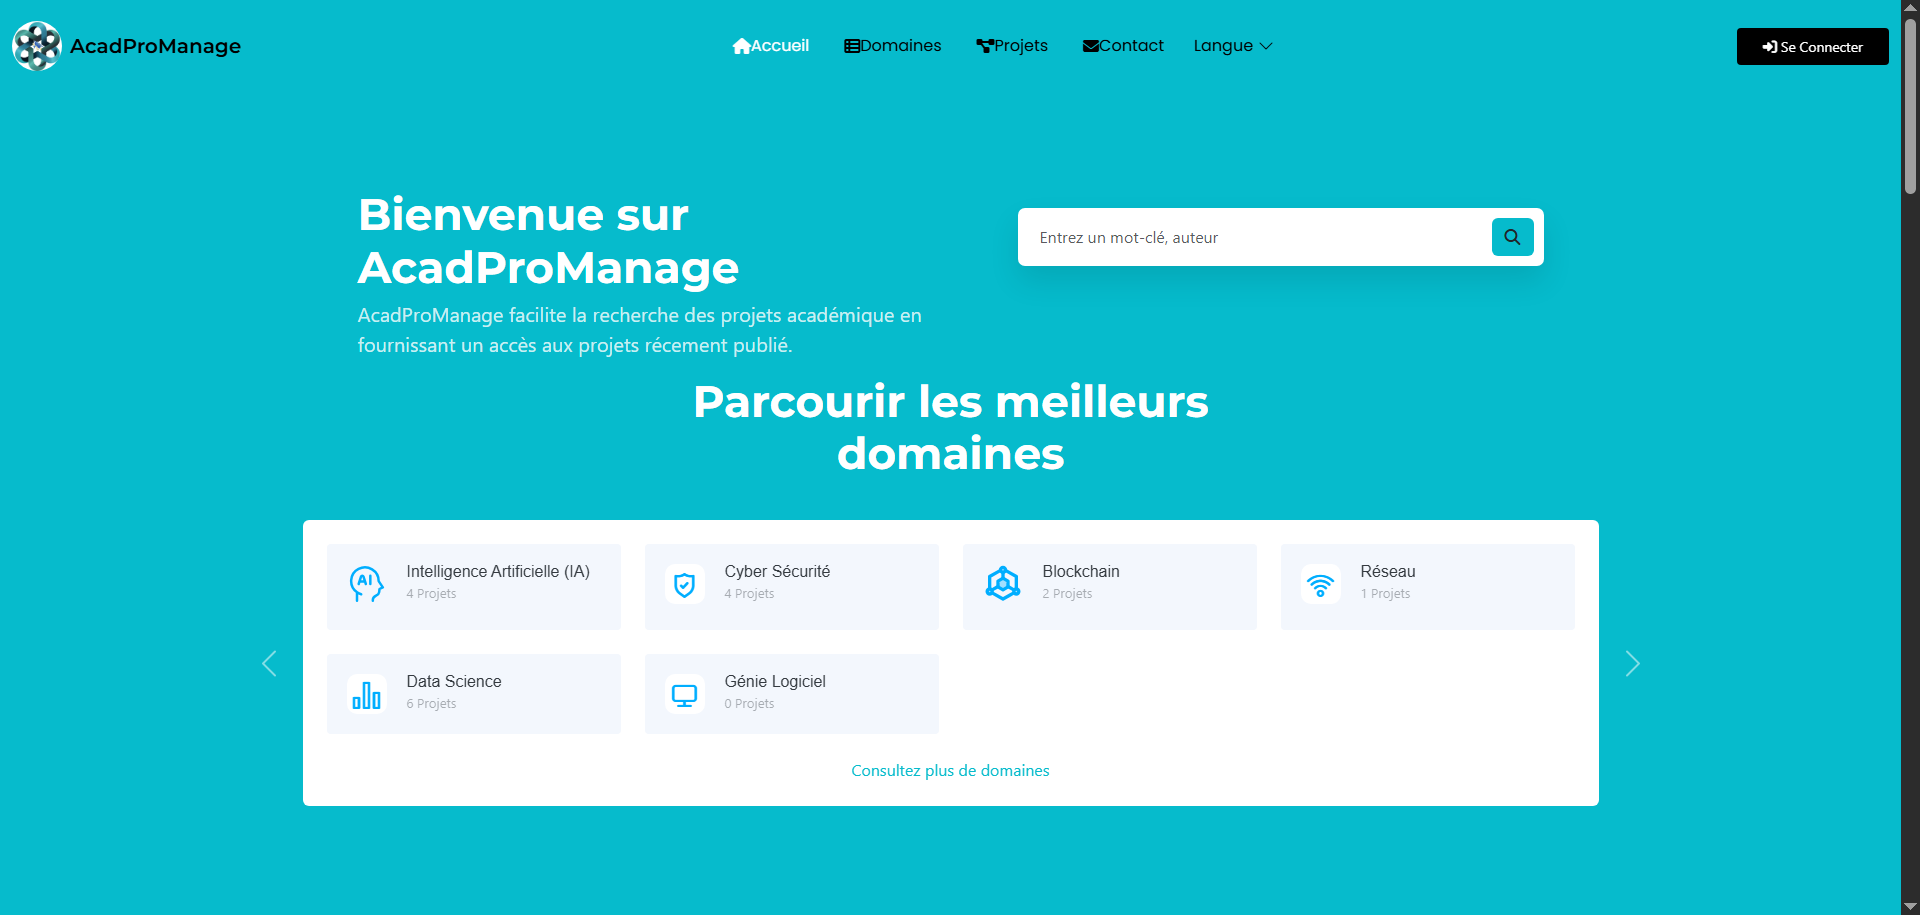
\includegraphics[width=0.7\textwidth]{./images/Accueil.png}
    \caption{Aperçu de la page d’accueil}
    \label{fig:Accueil}
\end{figure}

\medskip
En haut de cette page, vous trouverez des liens de redirection ("Accueil", "Domaines", "Projets", "Contact" et "Langue"). Ci-dessous sont présentées quelques fonctionnalités phares réalisables depuis cette page.
\medskip
\subsection{Rechercher des projets }
Pour ce faire, il faut saisir dans la barre de recherche un mot-clé, le nom d'un auteur ou d'un domaine.Vous serez ensuite rediriger vers la liste des projets relatifs au terme saisi. 
\medskip

\begin{figure}[h!]
    \centering
    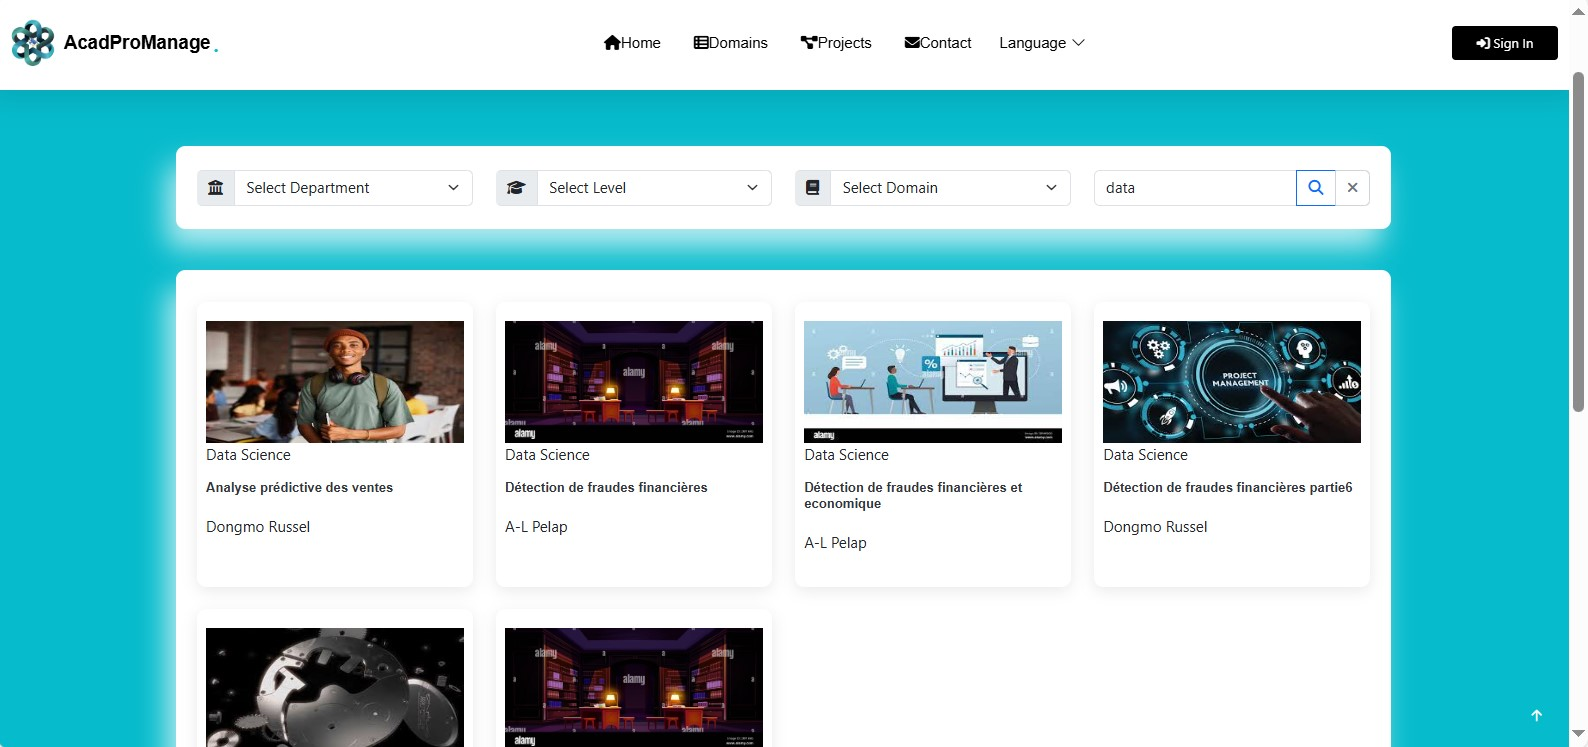
\includegraphics[width=0.7\textwidth]{./images/search-project.jpg}
    \caption{recherche d'un projet}
    \label{fig:recherche d'un projet}
\end{figure}

\medskip
\subsection{Rechercher un domaine d'étude }
La plateforme met en avant divers domaines telles que l'intelligence artificielle, la cybersécurité, la blockchain, la data science, le génie logiciel, etc. Pour y accéder, cliquez sur "Domains". Ainsi, vous aurez un visuel sur les domains étudiés, leur description et le nombre de projets y accordés.   
\medskip

\begin{figure}[h!]
    \centering
    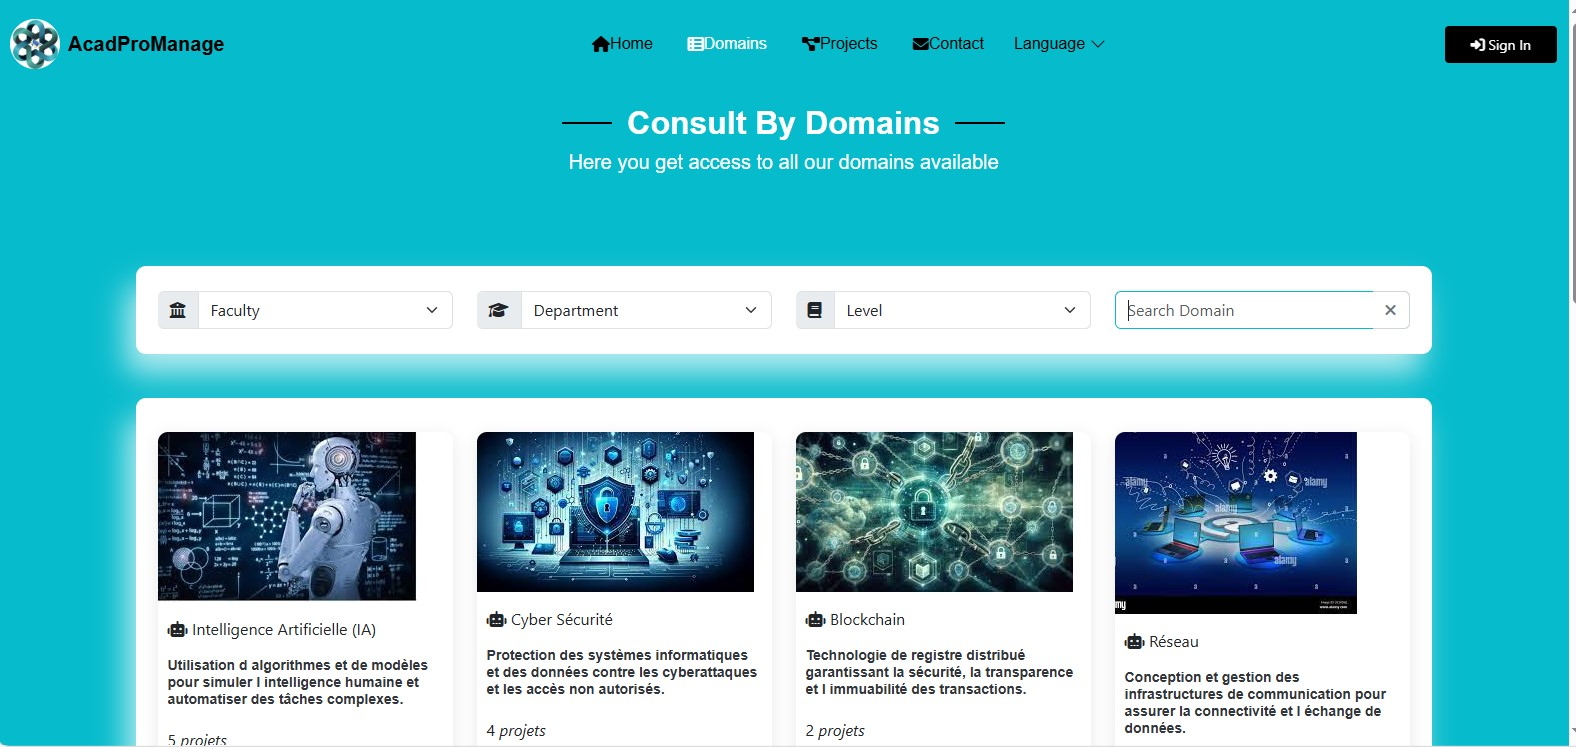
\includegraphics[width=0.8\textwidth]{./images/search-domain.jpg}
    \caption{recherche d'un domaine}
    \label{fig:recherche d'un domaine}
\end{figure}


\medskip
\subsection{Consulter les projets associés à un domaine spécifique}
Si un visiteur souhaite voir la liste des projets relatifs à un domaine en particulier(la cybersécurité, la blockchain, la data science, ou autres), il doit cliquer sur le domaine de son choix dans la liste des domaines ci-dessous. 
\medskip

\begin{figure}[h!]
    \centering
    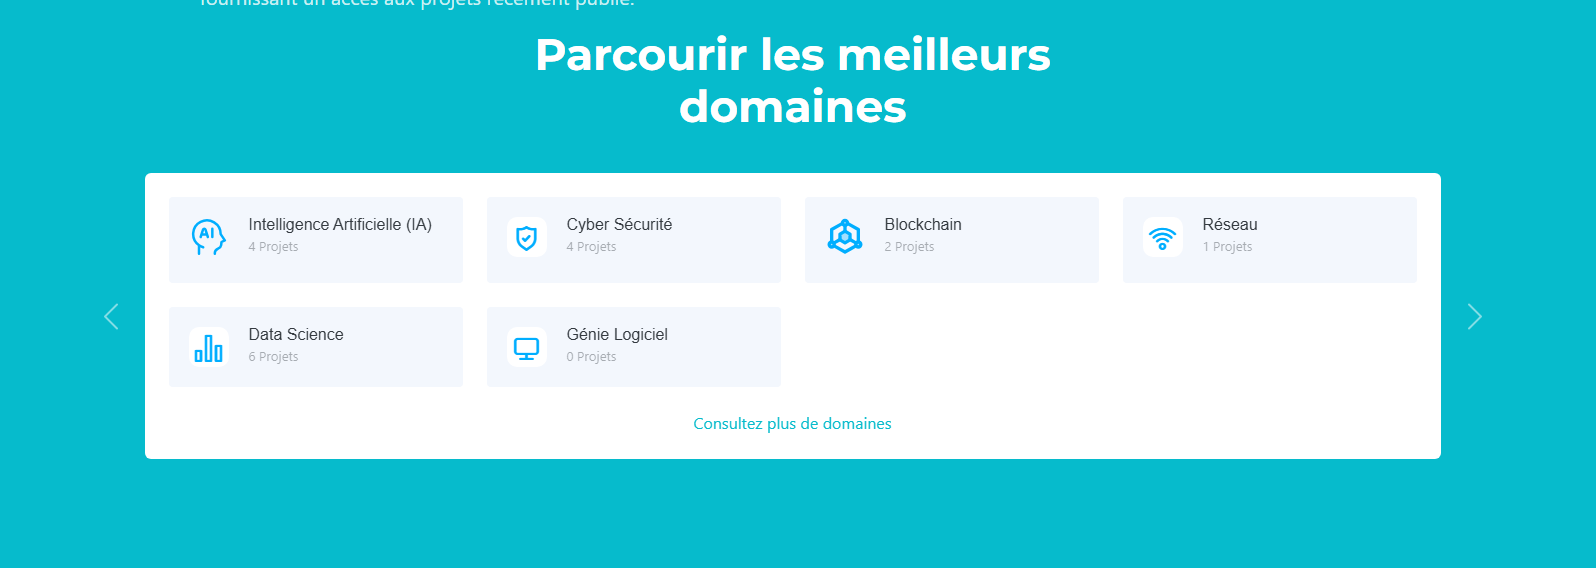
\includegraphics[width=0.8\textwidth]{./images/project-by-domain.png}
    \caption{consultation d'un projet}
    \label{fig:consultation d'un projet}
\end{figure}
\subsection{Se connecter}
Pour avoir un accès à votre espace personnel, cliquez sur "Sign in" ou "Se connecter" en haut à droite (en fonction de la langue que vous aurez choisie). Une pop-up s'affichera à cet effet, vous demandant de remplir vos informations personnelles dans les champs indiqués. Plusieurs cas de figures s'offrent à vous:

\medskip
\begin{figure}[h!]
    \centering
    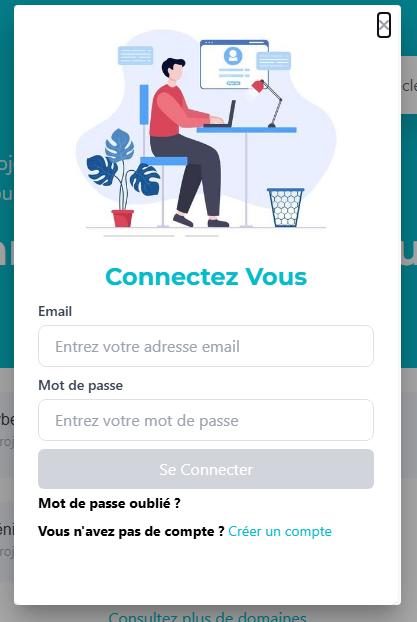
\includegraphics[width=0.3\textwidth]{./images/Connexion.png}
    \caption{page de connexion}
    \label{fig:page de connexion}
\end{figure}

\bigskip

\begin{itemize}
    \item Cliquez sur "Login" ou "Se connecter" si vous avez un compte. 
    \item Cliquez sur "Mot de passe oublié ?" si vous avez oublié votre mot de passe. Une pop-up vous proposera de fournir votre adresse e-mail pour la récupération de votre compte. Ceci fait,cliquez sur "Envoyer le code de vérification" pour valider. 
        \begin{figure}[h!]
            \centering
            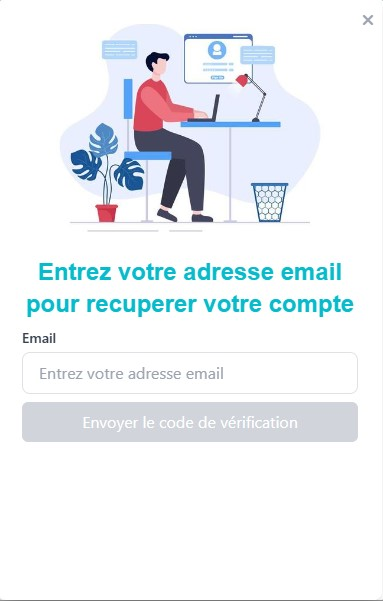
\includegraphics[width=0.3\textwidth]{./images/recup-compte.jpg}
            \caption{page de récupération de compte}
            \label{fig:page de récupération de compte}
        \end{figure}
    \item cliquez sur "Créer un compte" si vous n'avez pas de compte. Une pop-up s'ouvrira pour vous donner la possibilité de créer un compte. 
\end{itemize}
Lorsque la connexion aura réussie, vous aurez accès à un tableau de bord spécifique à votre fonction dans l'application.

\medskip

\subsection{Créer un compte}
La création d'un compte est une fonctionnalité sous-jacente à la connexion. Elle est régie par 02 étapes notamment:
\begin{itemize}
    \item Entrez vos informations personnelles ("nom, maticule, email, filière") dans les champs indiqués. Pour choisir une filière, cliquez sur le menu déroulant. Cliquez sur "Suivant" pour passer à l'étape 2. Voici un visuel:
            \begin{figure}[h!]
                \centering
                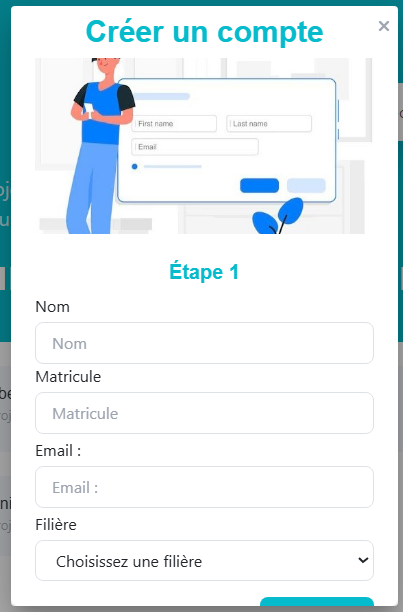
\includegraphics[width=0.18\textwidth]{./images/creercompte1.png}
                \caption{étape 1 de la création de compte}
                \label{fig:étape 1 de la création de compte}
            \end{figure}
        \medskip       
    \item Entrez votre mot de passe et confirmez-le. Cliquez sur "S'inscrire" pour finaliser la création de votre compte.
            \begin{figure}[h!]
                \centering
                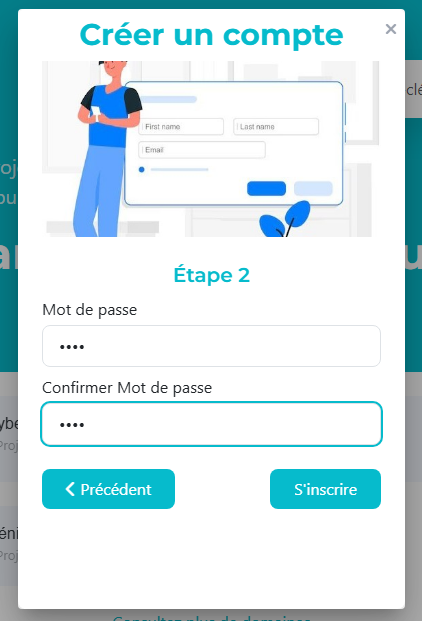
\includegraphics[width=0.2\textwidth]{images/creercompte2.png}
                \caption{étape 2 de la création de compte}
                \label{fig:etape2}
            \end{figure}
\end{itemize}
Pour revenir à l'étape précédente cliquez sur "Précédent".

\bigskip
\section{Fonctionnalités clés d'un utilisateur}
Une fois connecté, vous êtes dans votre tableau de bord. C'est d'ici que vous gérerez vos projets et votre profil. Vous serez accueillis par le message "Bienvenue dans votre espace personnel". Vous y trouverez diverses informations comme la liste détaillée de vos projets (elle est bien visible en-dessous du bouton "UPLOAD"), leurs statuts et une navigation vers des fonctionnalités supplémentaires. Sur le côté gauche, vous trouverez un menu de navigation vers les pages My Projects, Profile et Settings. Voici un exemple de tableau de bord utilisateur :

\begin{figure}[h!]
\centering
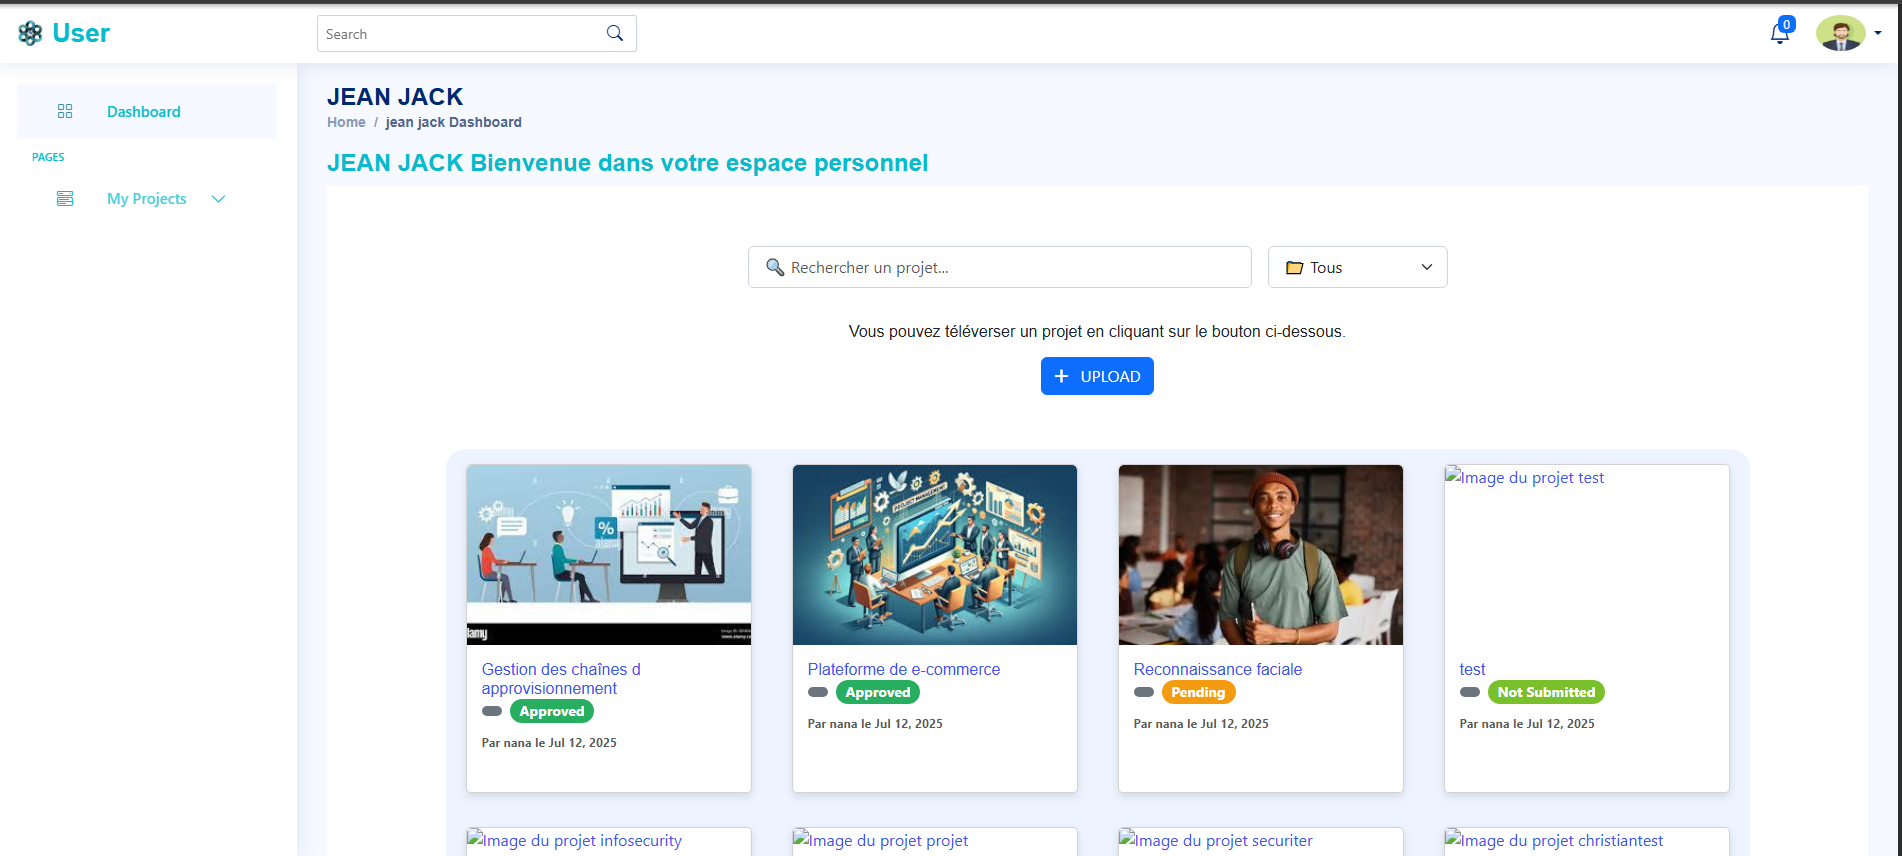
\includegraphics[width=0.5\textwidth]{images/dashboard-utilisateur .png}
\caption{Exemple de tableau de bord utilisateur}
\label{fig:dashboard user}
\end{figure}

\medskip
\subsection{Ajouter un Projet}
Depuis votre tableau de bord, vous avez la possibilité d’ajouter un nouveau projet. Pour cela, cliquez sur le bouton "+ UPLOAD" pour initier le processus de création d'un nouveau projet. Une fenêtre pop-up intitulée "Créer un projet" apparaîtra. Il vous suffira de suivre les trois étapes présentées. Elles sont entre autres:

\medskip
\subsubsection{Informations générales du projet}
Au cours de cette première étape,vous devez fournir des informations basiques concernant votre projet en remplissant les champs suivants:
\begin{itemize}
    \item Titre: Il correspond au titre de votre projet
    \item Type Projet: C'est un menu déroulant via lequel vous aurez accès aux types de projets. Choisissez celui qui vous convient le mieux.
    \item Couverture du projet: Ici vous devez cliquez sur le bouton "Choisir un fichier" pour désigner le fichier que vous souhaitez utiliser comme photo de couverture pour votre projet.
\end{itemize}
    Une fois terminé, cliquez sur le bouton "Next" pour passer à l'étape suivante.
  
\begin{figure}[h!]
    \centering
    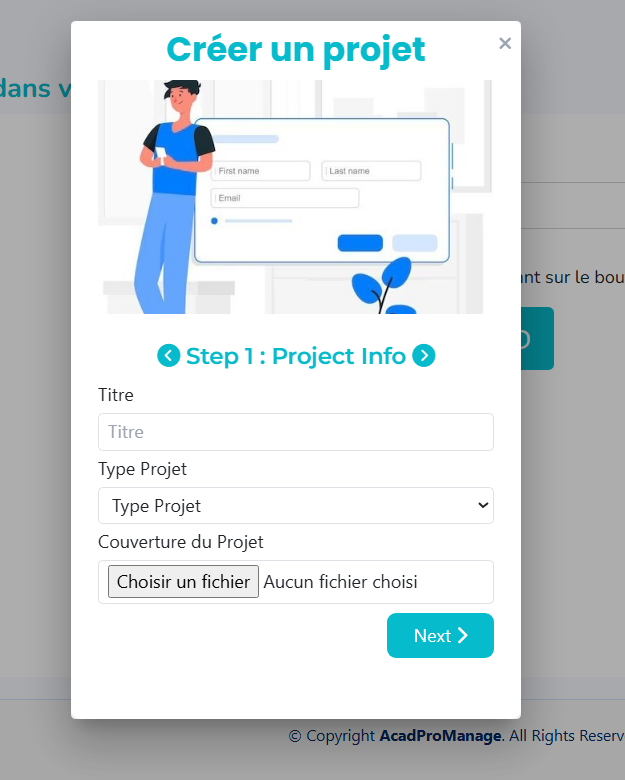
\includegraphics[width=0.4\textwidth]{./images/step1-create-project.png}
    \caption{première étape de création du projet}
    \label{fig:première étape de création du projet}
\end{figure}    

\smallskip
\subsubsection{Informations supplémentaires sur le projet}
Au cours de cette deuxième étape, vous devrez préciser le niveau et la catégorie de votre projet. Pour ce faire, vous devez remplir les champs:
\begin{itemize}
    \item Niveau: Il correspond à votre niveau d'étude académique lorsque vous soumettez le projet. Il peut prendre les valeurs Informatique1, Informatique3, et bien d'autres. Cliquez sur la flèche déroulante pour y accéder.
    \item Catégorie: Ici, vous devez renseigner la catégorie de votre projet. S'agit-il d'un projet sur l'Intelligence Artificielle? La cybersécurité ? Ou autre chose?
\end{itemize} 
Une fois terminé, cliquez sur le bouton "Next" pour passer à la prochaine étape.
Si vous souhaitez revenir à l'étape précédente, cliquez sur le bouton "Previous".

\begin{figure}[h!]
    \centering
    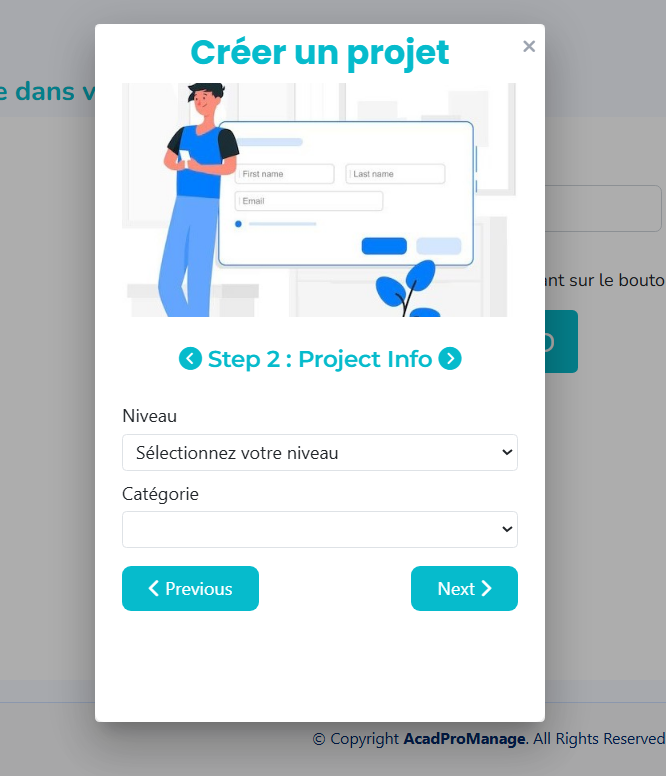
\includegraphics[width=0.3\textwidth]{./images/step2-create-project.png}
    \caption{deuxième étape de création du projet}
    \label{fig:deuxième étape de création du projet}
\end{figure}

\medskip
\subsubsection{Résumé du projet}
Vous devez dans la fenêtre qui s'affiche, dire en quelques mots ce dont traite votre projet. Vous devez fournir une description
pour votre projet. Une zone de saisie y est allouée. Pour rebrousser chemin, cliquez sur le bouton "Previous". Pour passer à la prochaine étape, utilisez le bouton "Next".

\begin{figure}[h!]
    \centering
    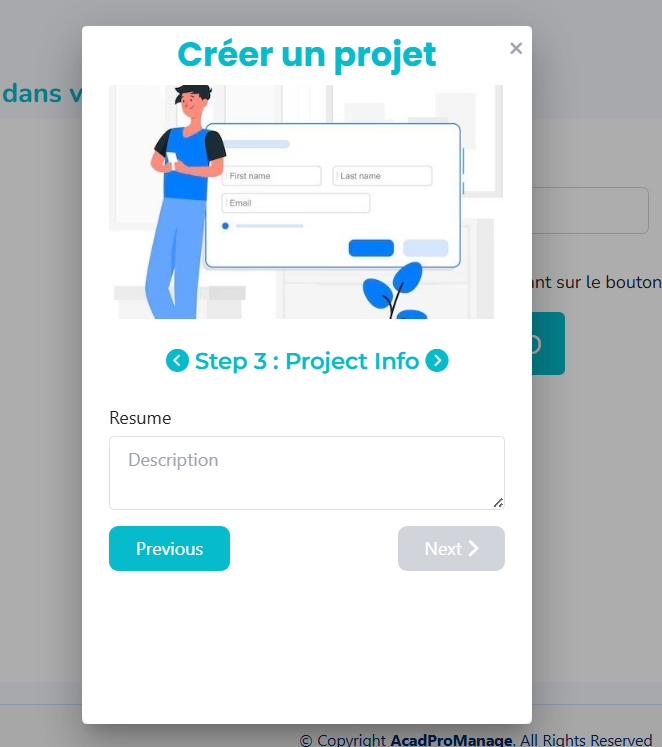
\includegraphics[width=0.3\textwidth]{./images/step3-create-project.png}
    \caption{troisième étape de configuration du projet}
    \label{fig:troisième étape de création du projet}
\end{figure}

\medskip
\subsubsection{Ajout d'un document}
Au sein de notre application, l'ajout de document est indispensable à la mise en ligne d'un projet. C'est une étape incontournable. Pour y parvenir, vous devezremplir les champs:
\begin{itemize}
    \item Nom du document: Vous pourrez, dans une zone réservée  à cet effet, fournir le nom que vous souhaitez adopter pour le document.
    \item Fichier : Vous devez cliquez sur le bouton "Choisir un fichier" pour importer le document de votre choix.
\end{itemize} 
Vous pourrez passer à la prochaine étape une fois fini.    

\begin{figure}[h!]
    \centering
    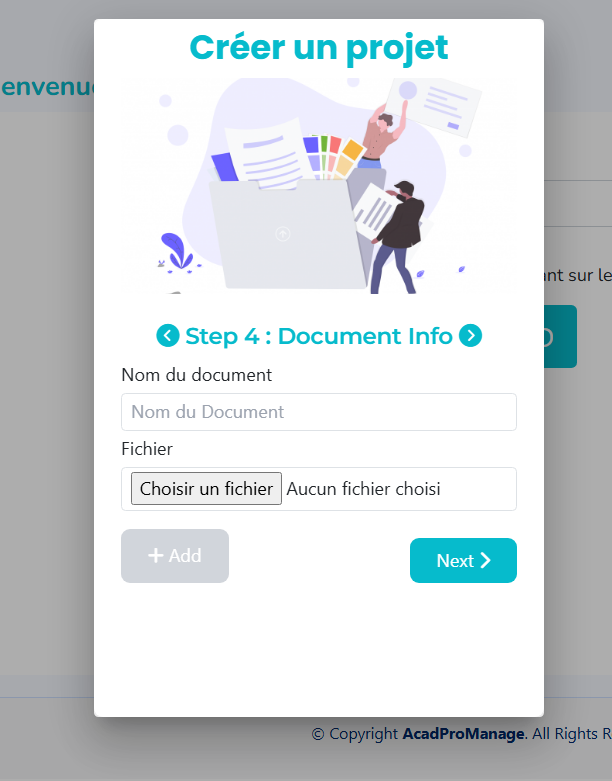
\includegraphics[width=0.25\textwidth]{./images/step4-create-project.png}
    \caption{quatrième étape de création d'un projet}
    \label{fig:quatrième étape de création du projet}
\end{figure}

\medskip
\subsubsection{Ajout d'un collaborateur sur le projet}
Ici, les collaborateurs sont les personnes avec lesquelles vous travaillez sur votre projet. Vous devrez fournir le nom et l'adresse email de vos collaborateurs. Cliquer sur "+ Add" autant de fois que vous ajouterez un collaborateur. Cliquez enfin sur "Next" pour passer aux informations du superviseur.
(NB : Cette étape n’est pas obligatoire dans la mesure ou vous êtes seul à travailler sur votre projet). Voici la fenêtre pour l'étape 4 de la création de projet :

\begin{figure}[h!]
\centering
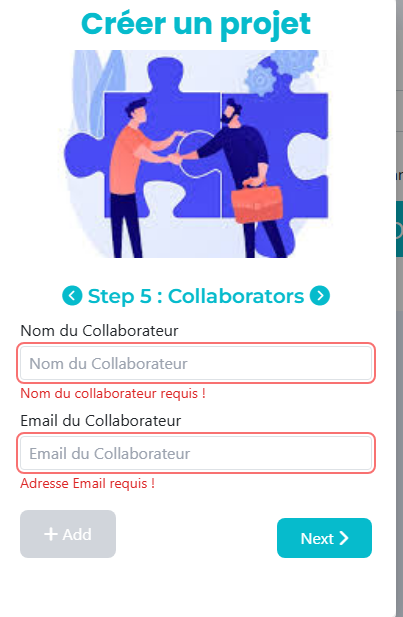
\includegraphics[width=0.25\textwidth]{images/etape5-projet.png}
\caption{cinquième étape de création du projet}
\label{fig:etape5projet}
\end{figure}

\medskip
\subsubsection{Ajout d'un superviseur au projet}
Ici, les superviseurs sont ceux qui ont la charge d'encadrer les étudiants. L'ajout d'un superviseur cloture le processus de création du projet. Dans les champs indiqués, vous devrez fournir les informations demandées sur le superviseur du projet. Cliquez sur "Finish" pour soumettre votre projet. Voici la fenêtre y associée:
\begin{figure}[h!]
\centering
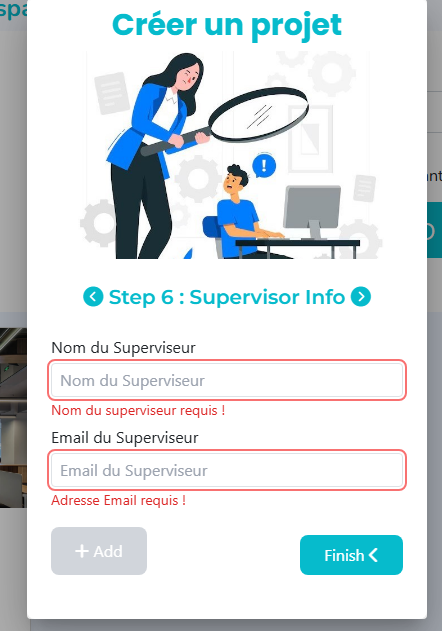
\includegraphics[width=0.3\textwidth]{images/etape6-projet.png}
\caption{ sixième étape de création du projet}
\label{fig:etape6projet}
\end{figure}
 
\bigskip
\subsection{Consulter la liste de ses projets}
Un utilisateur depuis son tableau de bord peut avoir accès à la liste des projets le concernant, qu'importe son rôle dans le système. Pour consulter globalement la liste de ses projets, il doit cliquer sur le menu déroulant "My Projects" situé à l'êxtreme gauche de son tableau de bord. Ici, seuls les noms des projets seront visibles. Voici l'un des rendus possibles:
    \begin{figure}[h!]
        \centering
        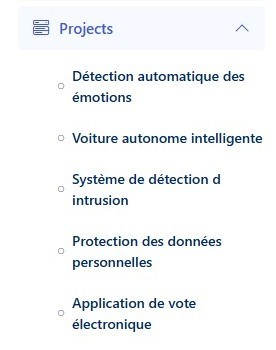
\includegraphics[width=0.3\textwidth]{images/min-project-list.jpg}
        \caption{liste des projets d'un utilisateur}
        \label{fig:liste des projets d'un utilsateur}
    \end{figure}

\bigskip
\subsection{Gérer les détails d'un projet}
Une fois votre projet créé, vous pouvez consulter et modifier les informations y relatives. Depuis votre tableau de bord, vous devez cliquer sur le projet en question pour le consulter. Vous devez garder à l'esprit que votre projet ne peut avoir plus d'un superviseur. Si vous interrompez le processus de création de votre projet avant la sixième étape, voici la page que vous verrez après clic sur le projet:

\begin{figure}[h!]
    \centering
    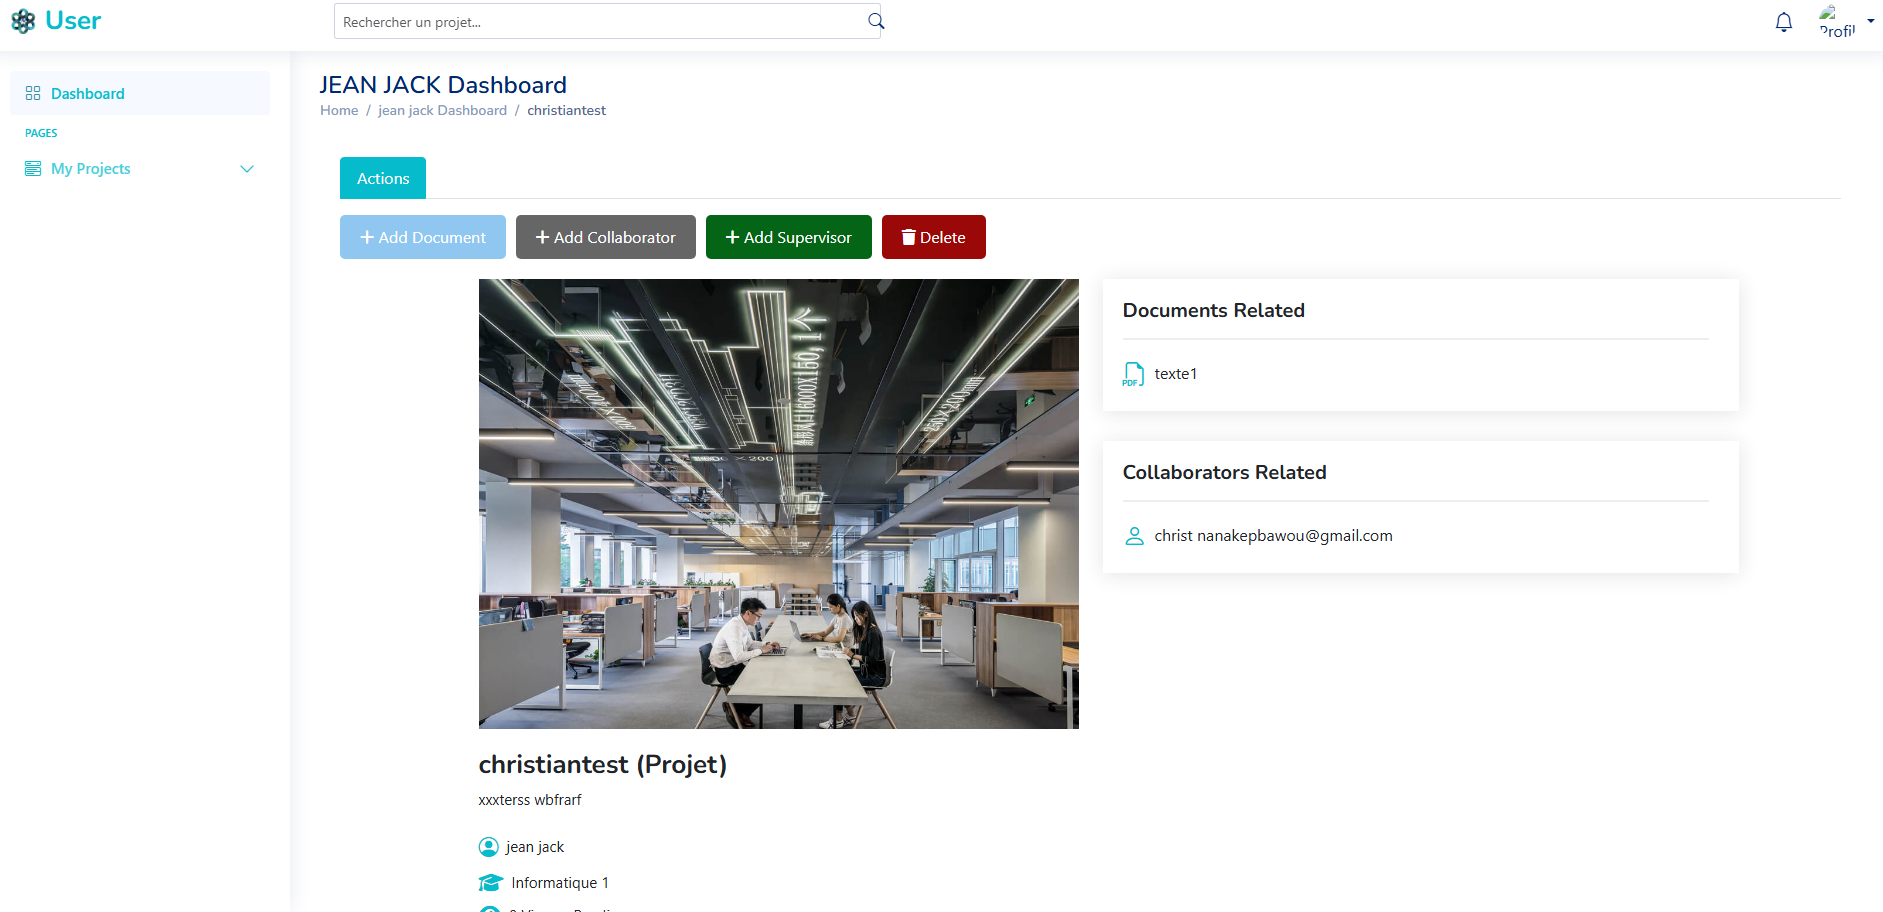
\includegraphics[width=0.8\textwidth]{./images/details-projet.png}
    \caption{vue détaillée d'un projet dans le tableau de bord d'un utilisateur}
    \label{fig:vue détaillée d'un projet chez un user}
\end{figure}

\medskip
De la figure précédente, on peut voir que plusieurs options s'offrent à nous notamment:
\begin{itemize}
    \item Ajouter un document: Pour cela, cliquez sur le bouton "Add Document" (à l'extrême gauche du menu Action). Une fenêtre nommée "Créer un document" s'ouvre, vous demandant de renseigner le nom du document. Cliquez ensuite sur "Choisir un fichier" pour sélectionner le document à importer. Cliquez enfin sur créer pour finaliser cette opération. Voici la fenêtre en question:
        \begin{figure}[h!]
            \centering
            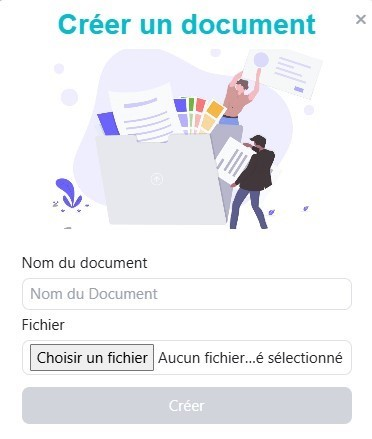
\includegraphics[width=0.4\textwidth]{./images/create-document.jpg}
            \caption{ajout d'un document à un projet existant}
            \label{fig:ajout d'un document pour un projet}
        \end{figure}
        
        \smallskip
        
    \item Ajouter un collaborateur: L'ajout d'un collaborateur se fait par clic sur le bouton "Add Collaborator". La fenêtre "Add Collaborator" s'affiche. Vous devez fournir les informations demandées. Cliquez sur Ajouter pour terminer. Voici la page y relative:
        \begin{figure}[h!]
            \centering
            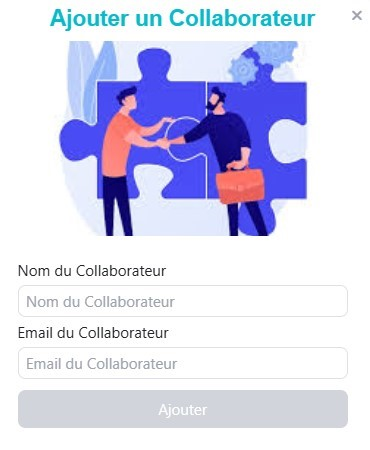
\includegraphics[width=0.4\textwidth]{./images/add-collaborator.jpg}
            \caption{ajout d'un collaborateur à un projet existant}
            \label{fig:ajout d'un collaborateur à un projet existant}
        \end{figure}
        
        \medskip

    \item Choisir un superviseur: Ce choix se fait par clic sur le menu déroulant "Choose Supervisor". Il fournit une liste de superviseurs dont les noms et adresses sont fournies. Vous pourrez sélectionner celui qui vous convient. Cliquez ensuite sur le bouton "Assigner le superviseur sélectionné". Une pop-up s'affiche lorsque cette opération aboutit.
        \begin{figure}[h!]
            \centering
            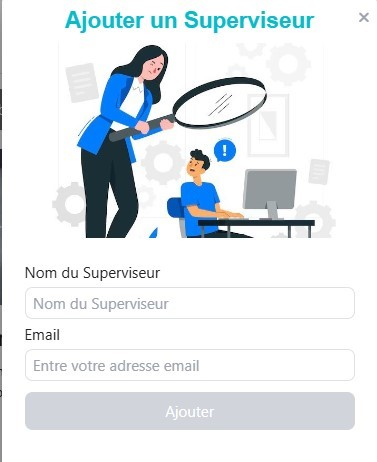
\includegraphics[width=0.4\textwidth]{./images/add-supervisor.jpg}
            \caption{ajout d'un superviseur à un projet existant}
            \label{fig:ajout d'un superviseur à un projet existant}
        \end{figure}
        
        \medskip

    \item Supprimer le projet: Si vous souhaitez vous débarrasser de votre projet, vous devez cliquer sur le bouton "Delete". Une pop-up de validation s'affichera. Cliquez sur "Yes" pour confirmer ou sur "Cancel" pour annuler. Voici ladite pop-up:
        \begin{figure}[h!]
            \centering
            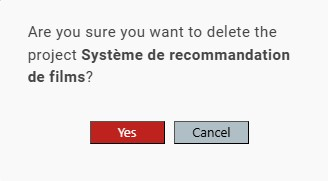
\includegraphics[width=0.4\textwidth]{./images/delete-project.jpg}
            \caption{suppression d'un projet existant}
            \label{fig:suppression d'un projet existant}
        \end{figure}

       \medskip
    \item Supprimer un document: Si vous voulez supprimer un document, cliquez sur l'icône de poubelle (en rouge) à côté du document que vous souhaitez retirer du projet. Une pop-up de confirmation s'ouvre alors. Cliquez sur "Ok" pour valider.     
\end{itemize}

\medskip
\subsection{Gérer son profil}
Tout utilisateur, depuis son tableau de bord peut avoir une vue d'ensemble sur ses informations personnelles. Il peut en outre les visualiser ou les modifier. Vous pourrez ainsi maintenir vos coordonnées à jour.
Voici quelques actions que vous pouvez effectuer sur votre profil:

\medskip
\subsubsection{Visualiser son profil}
Pour accéder à votre profil, vous devez cliquez sur "Profile" situé dans le menu déroulant en haut à droite (sous votre nom d'utilisateur). L'image suivante apparaîtra: 
\medskip

\begin{figure}[h!]
\centering
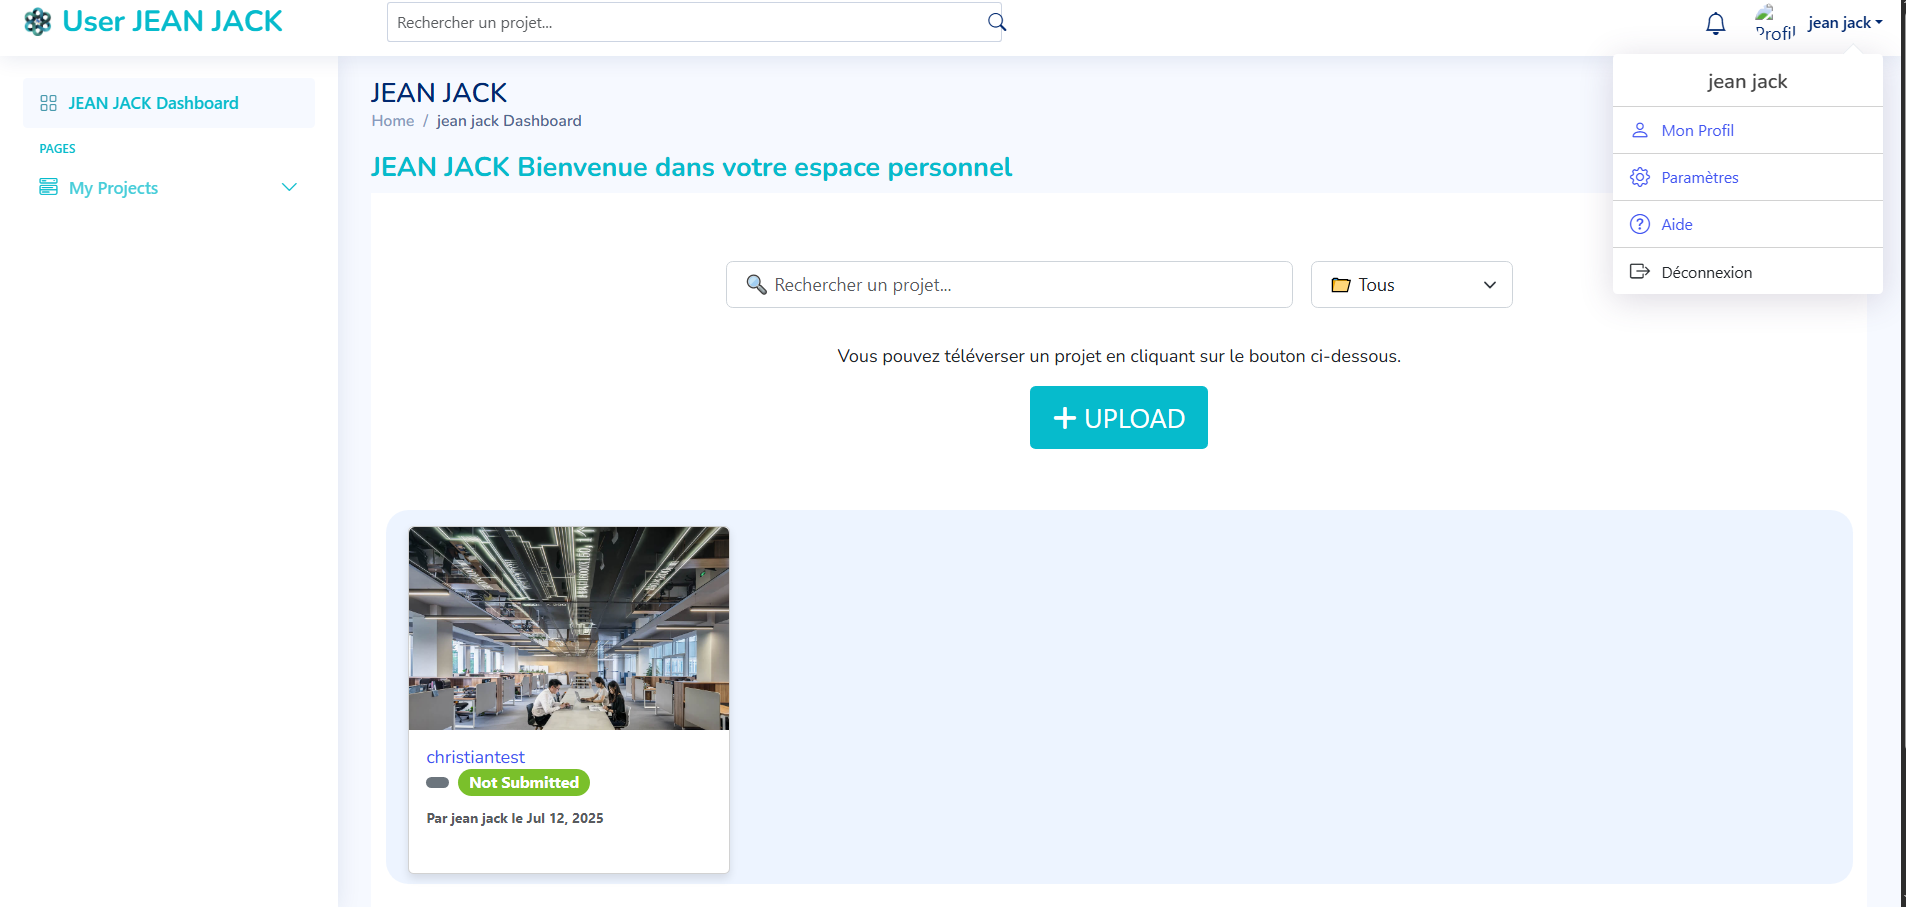
\includegraphics[width=0.5\textwidth]{./images/profile-access.png}
\caption{accès au profil}
\label{fig:accès au profil}
\end{figure}

\medskip
\subsubsection{Modifier son profil}
Une fois votre profil ouvert, vous pouvez modifier vos informations à votre guise. Parmi ces informations figurent votre nom, votre prénom, votre email, votre mot de passe et enfin votre photo. Voici les directives à suivre en fonction du bouton sur lequel vous cliquerez:
\medskip
\begin{itemize}
\item Modifier Nom/Prénom: Vous devez saisir vos nouveaux nom et prénom dans les champs spécifiques. Cliquez ensuite sur le bouton "Enregistrer" lorsque vous aurez fini. Voici le fenêtre qui s'affiche pour cet ajustement.
    \begin{figure}[h!]
        \centering
        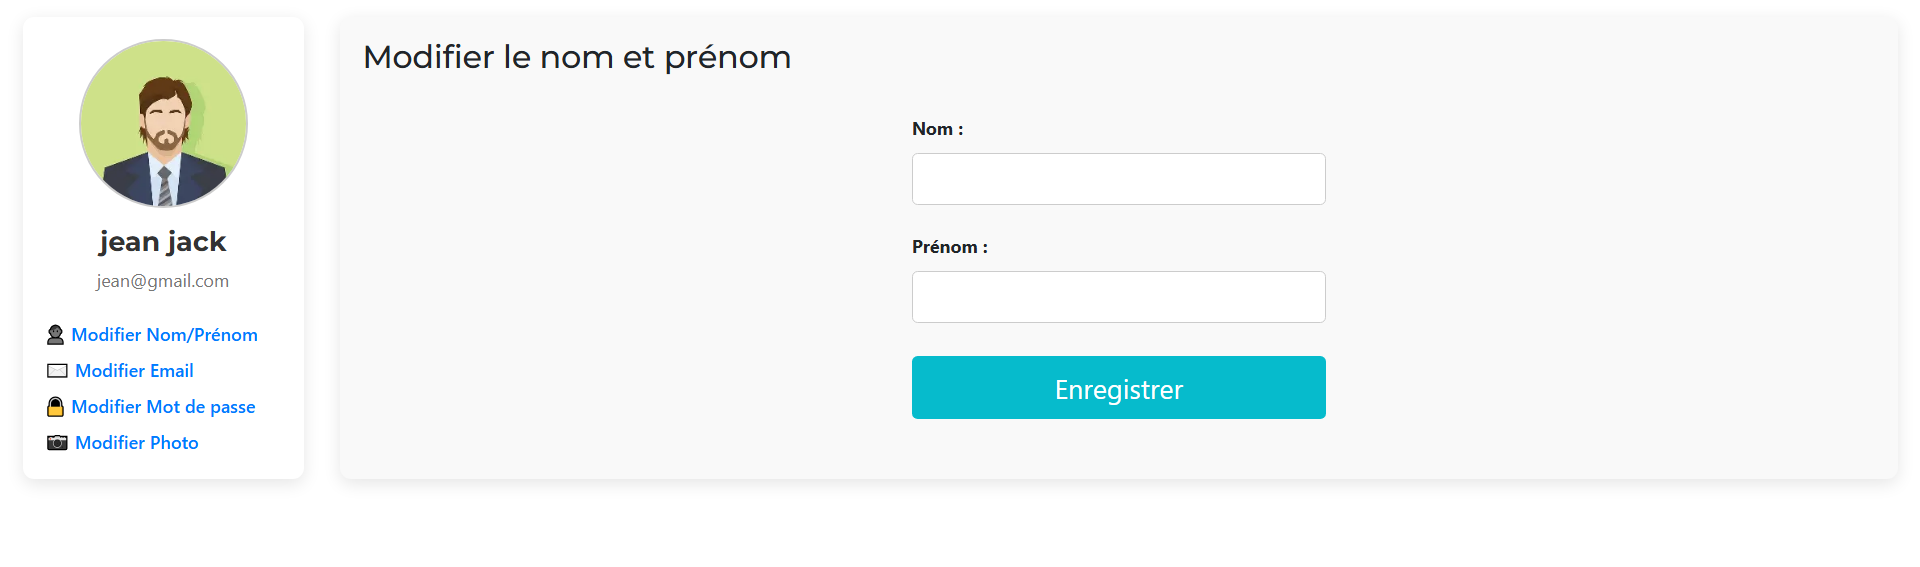
\includegraphics[width=0.6\textwidth]{./images/modify-profile-name.png}
        \caption{modification du Nom/Prénom}
        \label{fig:modification du Nom/Prénom}
    \end{figure}
    
\item Modifier Email: Vous devez saisir votre nouvelle adresse email dans le champ spécifique. Cliquez ensuite sur le bouton "Enregistrer" pour sauvegarder cette modification. Voici le fenêtre qui s'affiche pour cet ajustement.
    \begin{figure}[h!]
        \centering
        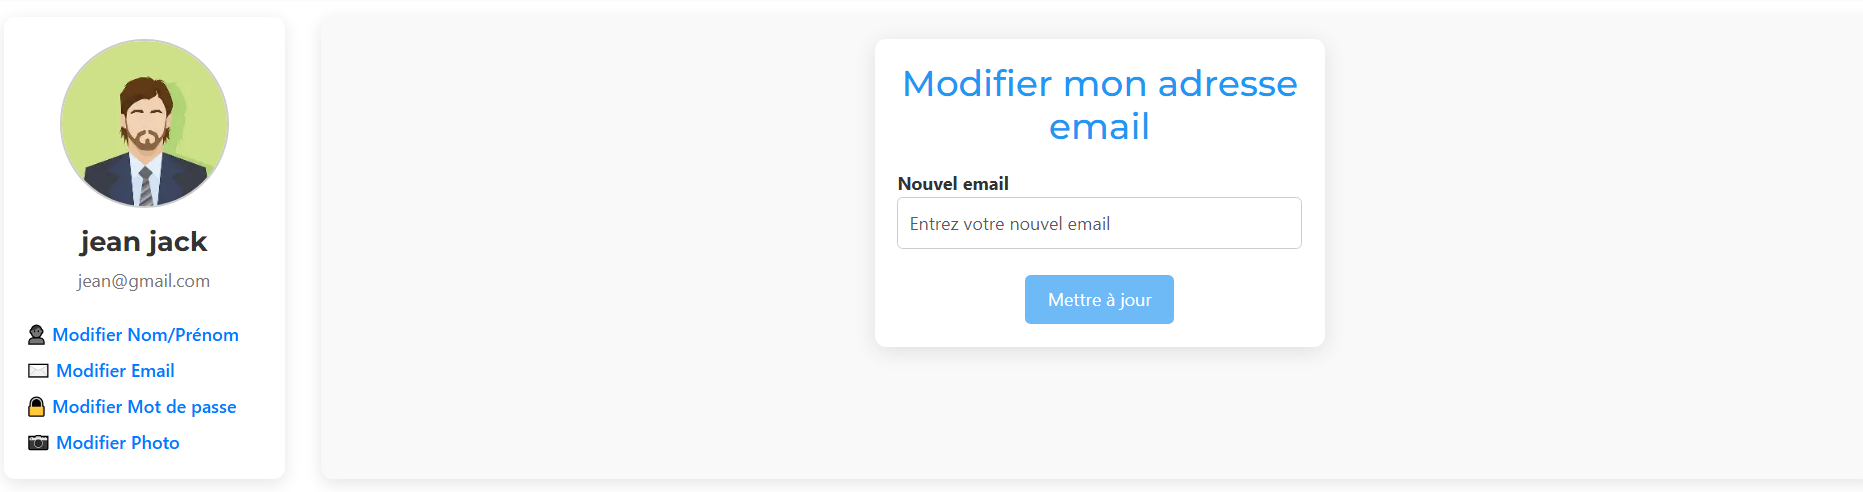
\includegraphics[width=0.6\textwidth]{./images/modify-email.png}
        \caption{modification de l'email}
        \label{fig:modification de l'email}
    \end{figure}
\item Modifier Mot de passe: Vous devez saisir votre mot de passe actuel dans le champ  "ancien mot de passe"  et le mot de passe que vous souhaitez utiliser dans le champ  "nouveau mot de passe" . Cliquez sur le bouton "Enregistrer" pour sauvegarder cette modification. Voici la fenêtre y relative:
    \begin{figure}[h!]
        \centering
        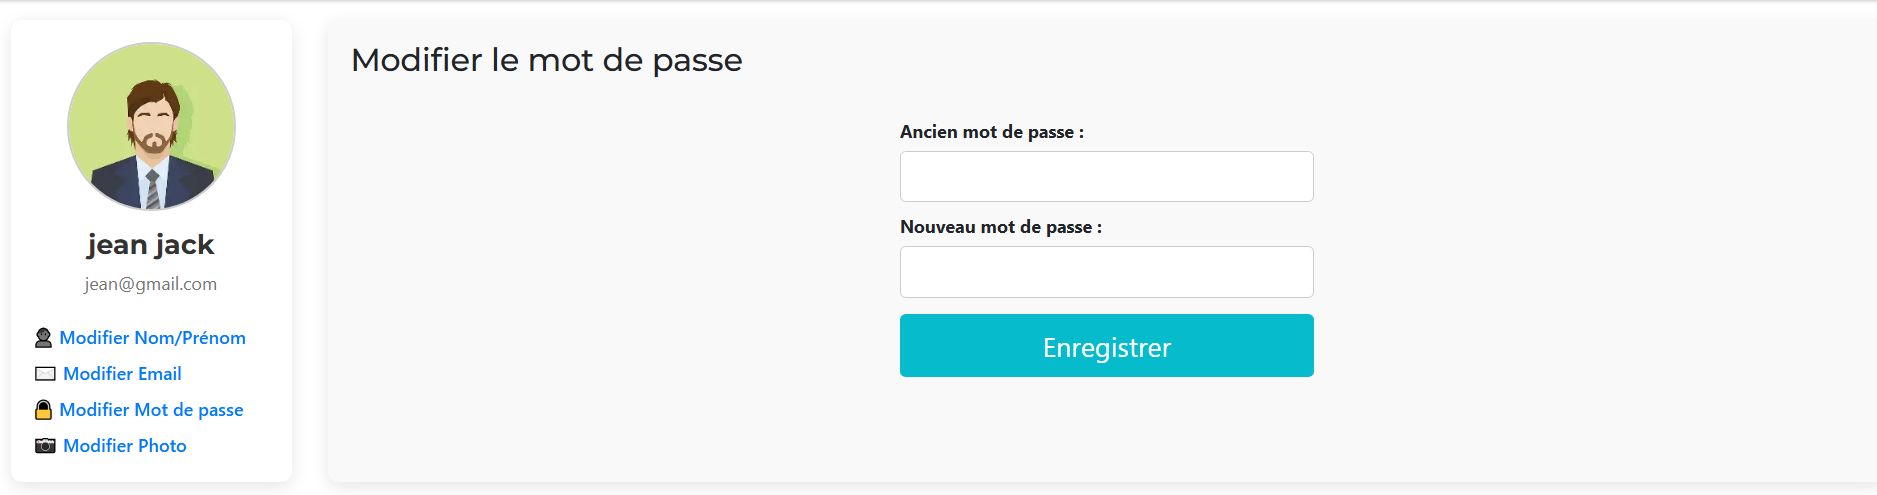
\includegraphics[width=0.6\textwidth]{./images/modify-password.png}
        \caption{modification du mot de passe}
        \label{fig:modification du mot de passe}
    \end{figure}
\item Modifier Photo: Pour choisir une nouvelle photo, cliquez sur l'icone en forme de caméra située sur l'image du profil(au-dessus du bouton "Enregistrer", dans la partie droite de la page). Après avoir cliqué sur la photo de votre choix, cliquez sur le "Ouvrir" puis sur le bouton "Enregistrer" pour valider. Voici le fenêtre pour cette modification:
    \begin{figure}[h!]
        \centering
        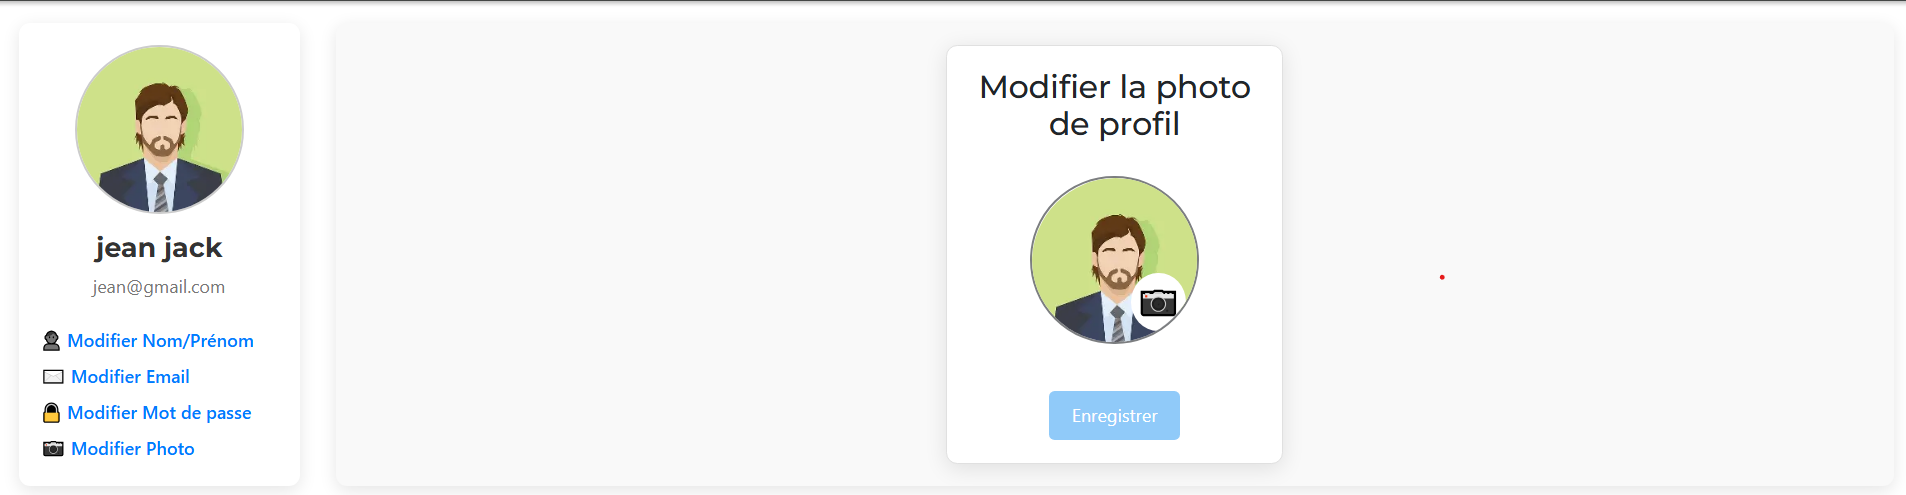
\includegraphics[width=0.6\textwidth]{./images/modify-photo.png}
        \caption{modification de la photo}
        \label{fig:modification de la photo}
    \end{figure}
\end{itemize}

\bigskip
\subsection{Se déconnecter}
Lorsqu'un utilisateur n'a plus besoin de rester en ligne ou souhaite revenir à la page d'accueil, il effectue un déconnexion pour y parvenir. Depuis votre tableau de bord, vous devez cliquer sur votre nom d'utilisateur en haut à droite, puis choisir l'option "Déconnexion" dans le menu déroulant. Cliquez ensuite sur "OK" dans la fenêtre pop-up qui s'affichera. Vous serez rediriger vers la page d'accueil. Voici une vue sur la déconnexion d'un utilisateur.

    \begin{figure}[h!]
            \centering
            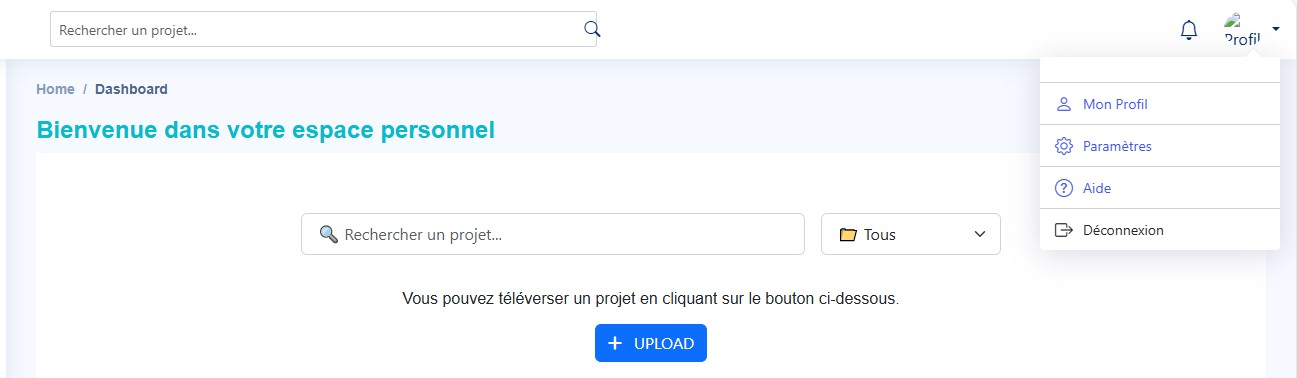
\includegraphics[width=0.6\textwidth]{./images/deconnexion-user.jpg}
            \caption{déconnexion d'un utilisateur}
            \label{fig:déconnexion d'un utilisateur}
    \end{figure}

\bigskip    
\section{Fonctionnalités pour un superviseur}
Afin de sauvegarder les informations relatives au monitoring des projets, AcadPromanage prévoit la mise en place de superviseurs. Dans notre cas particulier, un superviseur joue le rôle d'un enseignant au sein d'un projet. Dans son tableau de bord, il a une vue globale sur ses projets (Approuvés : 17, En attente : 7, Rejetés : 9), accès à la liste de ses projets et plus encore. Voici un visuel de son tableau de bord:
    \begin{figure}[h!]
        \centering
        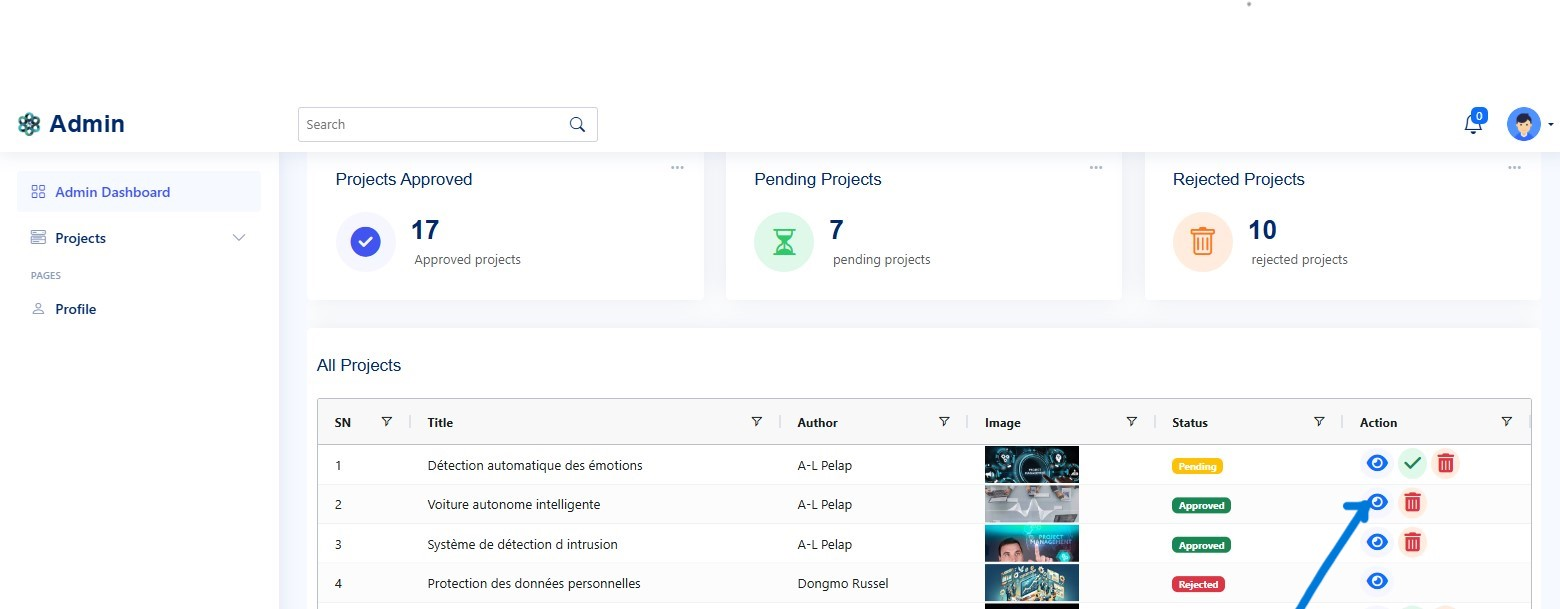
\includegraphics[width=0.6\textwidth]{images/admin-dashboard.jpg}
        \caption{Exemple de tableau de bord superviseur}
        \label{fig:dashboard enseignant}
    \end{figure}

Un superviseur peut alors valider un projet, le rejeter ou le mettre en attente. En outre, en tant qu'utilisateur du système, il peut se connecter/déconnecter, consulter ses projets(ceux lui ayant été soumis) et bien évidemment gérer son profil. Voici comment se présente la modification du statut d'un projet:

\bigskip
Pour modifier le statut d'un projet, le superviseur doit cliquer sur l'oeil bleu (pour avoir accès à la page détaillant le projet) situé dans la zone "Action" de la liste exhaustive de ses projets. Voici l'emplacement de ce bouton:
\begin{figure}[h!]
        \centering
        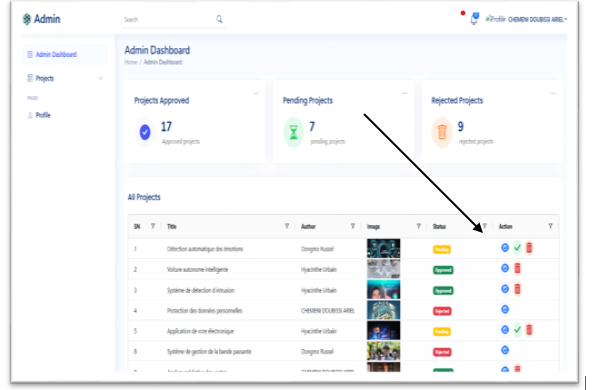
\includegraphics[width=0.5\textwidth]{images/image_tri_tableau.png}
        \caption{emplacement du bouton de mofification du statut d'un projet}
        \label{fig:bouton de mofification du statut d'un projet}
    \end{figure}

    La "flèche verte" indique que le projet peut être approuvé. La "poubelle rouge" indique que le projet peut être rejeté(s'il était en attente) ou mis en attente(s'il était approuvé). Aucun projet ne peut être approuvé ou rejeté sans passer par une mise en attente. Voici quelques indications sur la modification du statut d'un projet:
    \begin{itemize}
    \item approuvé à mis en attente
    \item rejeté à mis en attente
    \item mis en attente à approuvé
    \item mis en attente à rejeté
    \end{itemize}  

\medskip
Après clic sur l'oeil, une page détaillée sur le projet s'affiche. Nous verrons ces différentes pages en fonction du statut du projet actuel. 

\medskip
\subsection{Approuver un projet}
Voici la page qui s'affiche pour un projet en attente:
    \begin{figure}[h!]
        \centering
        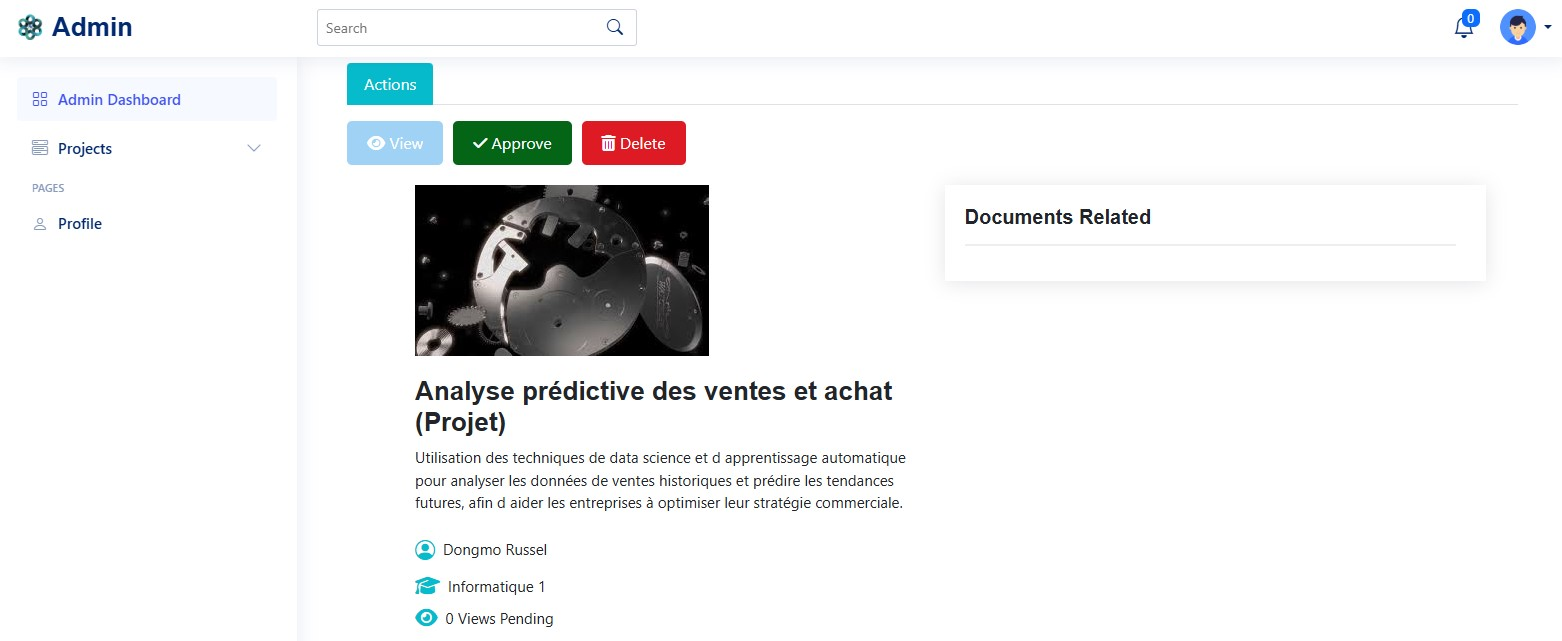
\includegraphics[width=0.7\textwidth]{images/project-pending-R.jpg}
        \caption{vue sur un projet en attente}
        \label{vue sur un projet en attente}
    \end{figure}

Pour approuver ce projet, il faut cliquer sur le bouton "Approve" (en vert) dont la position a été repérée sur l'image précédente. Dès lors, une pop-up s'affiche vous demandant d'attester de l'approbation du projet. Cliquez sur "Ok" pour valider. Suite à cela, le projet prendra le statut "Approved". Voici le rendu depuis le dashbord lorsque que cette opération porte ses fruits: 
    \begin{figure}[h!]
        \centering
        
\includegraphics[width=0.8\textwidth]{images/pending-project-R.jpg}
        \caption{vue sur le dashboard avant l'approbation d'un projet en attente}
        \label{dashboard avant approbation d'un projet en attente}
    \end{figure}

\medskip

    \begin{figure}[h!]
        \centering
        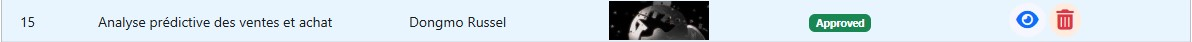
\includegraphics[width=0.8\textwidth]{images/approved-project-R.jpg}
        \caption{vue sur le dashboard après l'approbation d'un projet en attente}
        \label{dashboard après approbation d'un projet en attente}
    \end{figure}


\medskip
\subsection{Rejeter un projet}
Comme vu précédemment, seuls les projets en attente peuvent être rejetés. Nous nous appuyerons donc sur la même image que celle de l'approbation pour que vous puissiez clairement voir la différence. 
Pour rejeter ce projet, il faut cliquer sur le bouton "Delete" (en rouge) dont la position est connue. Dès lors, une pop-up s'affiche vous demandant d'attester du rejet du projet en question. Cliquez sur "Ok" pour valider. Suite à cela, le projet prendra le statut "Rejected". Voici le rendu depuis le dashbord lorsque cette opération est un franc succès: 
    \begin{figure}[h!]
        \centering
        
\includegraphics[width=0.8\textwidth]{images/pending-project-R.jpg}
        \caption{vue sur le dashboard avant le rejet d'un projet en attente}
        \label{dashboard avant le rejet d'un projet en attente}
    \end{figure}

\medskip

    \begin{figure}[h!]
        \centering
        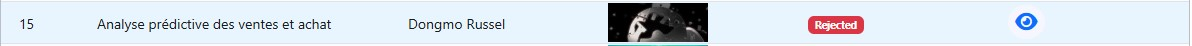
\includegraphics[width=0.8\textwidth]{images/project-rejected-R.jpg}
        \caption{vue sur le dashboard après rejet d'un projet en attente}
        \label{dashboard après rejet d'un projet en attente}
    \end{figure}

\medskip
\subsection{Mettre en attente un projet}
Il faut noter que, dès lors qu'un projet est soumis, son statut par défaut est "en attente". À présent, nous verrons comment mettre manuellement les projets soumis en attente. Deux cas de figures sont à distinguer:

\subsubsection{Mettre en attente un projet approuvé}
Lorsque vous souhaitez rejeter un projet précédemment approuvé, vous devez d'abord le mettre en attente. Pour cela, il faut cliquer sur le bouton "Restore" (en rouge) dans la page détail du projet. Alors, une pop-up s'affiche vous demandant si vous souhaitez mettre en attente ledit projet. Cliquez sur "Ok" pour accepter. Après cela, le projet prendra le statut "Pending". Ci-dessous sont présentées la vue du projet approuvé dans la page détaillant le projet, ainsi que les modifications depuis le dashbord avant et après changement du statut du projet. 
        \begin{figure}[h!]
            \centering
            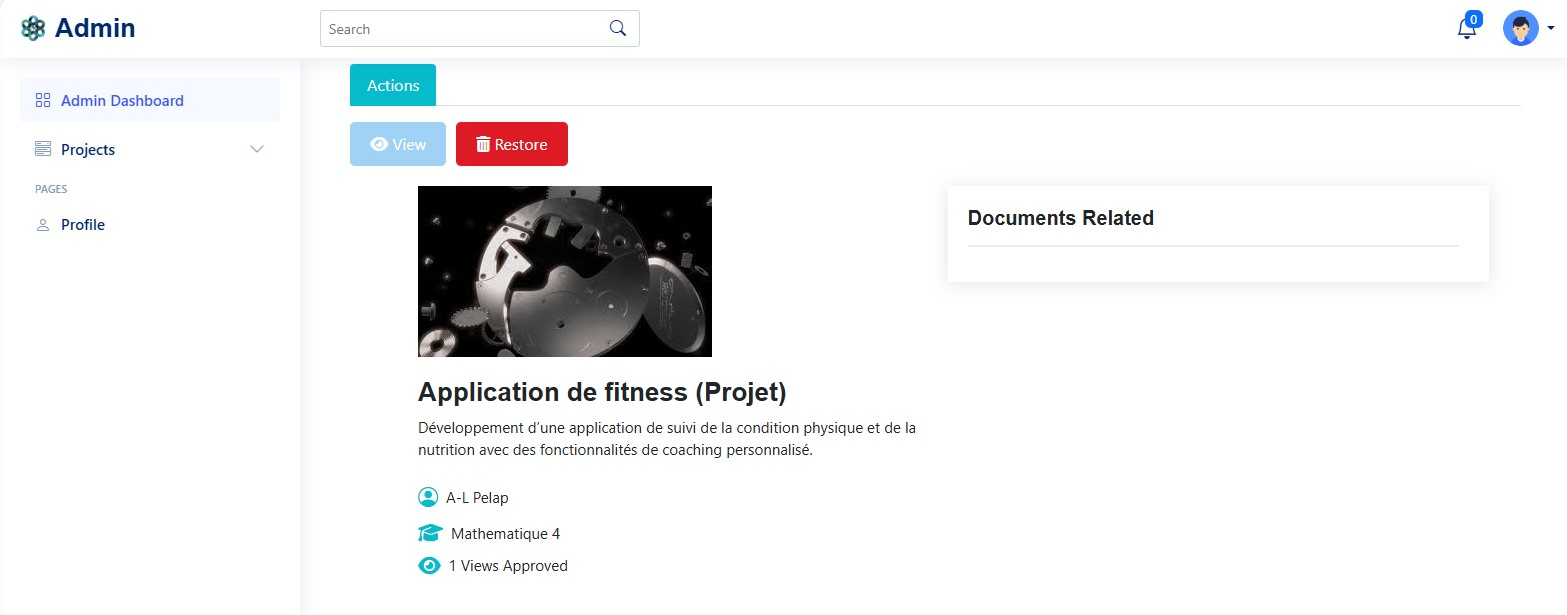
\includegraphics[width=0.8\textwidth]{images/project-approved-A.jpg}
            \caption{vue sur un projet approuvé}
            \label{vue sur un projet approuvé}
        \end{figure}

    \medskip

        \begin{figure}[h!]
            \centering
            
\includegraphics[width=0.8\textwidth]{images/approved-project-A.jpg}
            \caption{vue sur le dashboard avant la mise en attente d'un projet approuvé}
            \label{dashboard avant mise en attente pour projet approuvé}
        \end{figure}

    \medskip

        \begin{figure}[h!]
            \centering
            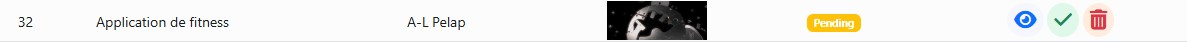
\includegraphics[width=0.8\textwidth]{images/pending-project-A.jpg}
            \caption{vue sur le dashboard après mise en attente d'un projet approuvé}
            \label{dashboard après mise en attente d'un projet approuvé}
        \end{figure}

    \medskip
\newpage
\subsubsection{Mettre en attente un projet rejeté}
Lorsque vous annulez le rejet d'un projet, on parle de restauration du projet. Dans ce cas, vous devez cliquer sur le bouton "Restore" (en vert) dans la page détail du projet. Alors, une pop-up s'affiche vous demandant si vous souhaitez mettre ce projet à l'état de mise en attente. Cliquez sur "Ok" pour accepter. Après cela, le projet prendra le statut "Pending". Ci-dessous sont présentées la vue du projet rejeté dans la page détaillant le projet, ainsi que les modifications depuis le dashbord avant et après changement du statut du projet. 
        \begin{figure}[h!]
            \centering
            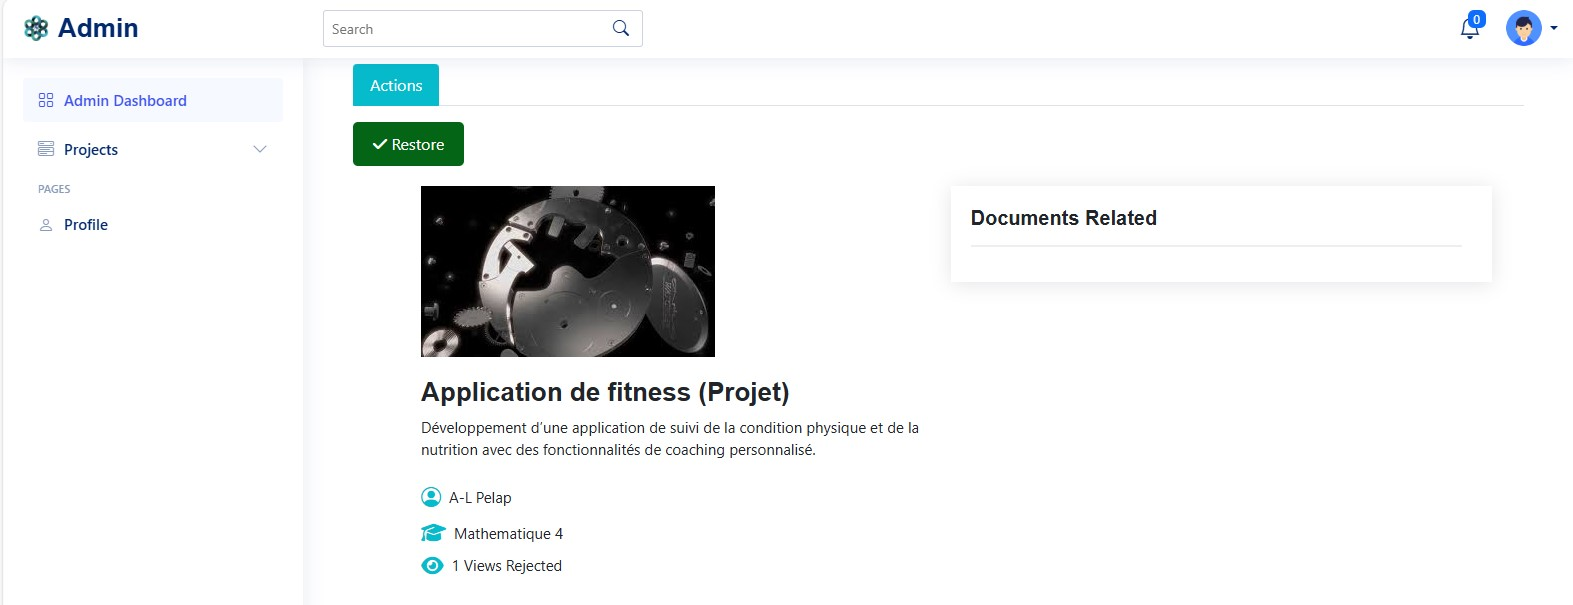
\includegraphics[width=0.8\textwidth]{images/restore-reject-project-A.jpg}
            \caption{vue sur un projet rejeté}
            \label{vue sur un projet rejeté}
        \end{figure}
    \smallskip
        \begin{figure}[h!]
            \centering
            
\includegraphics[width=0.8\textwidth]{images/rejected-project-A.jpg}
            \caption{vue sur le dashboard avant la mise en attente d'un projet rejeté}
            \label{dashboard avant mise en attente pour projet rejeté}
        \end{figure}
    \medskip
        \begin{figure}[h!]
            \centering
            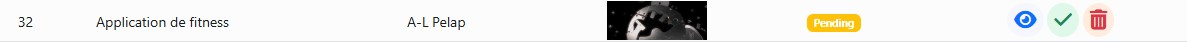
\includegraphics[width=0.8\textwidth]{images/pending-project-A.jpg}
            \caption{vue sur le dashboard après mise en attente d'un projet rejeté}
            \label{dashboard après mise en attente d'un projet rejeté}
        \end{figure}

\newpage
\section{Alternatives pour les utilisateurs}
Si tout au long du parcours de ce manuel vous ressentez des incompréhensions ou nourrissez des incertitudes, notre plateforme reste à votre entière disposition. À cet effet, nous prévoyons la mise en place d'une page d'aide qui vous est totalement dévouée. Elle est accessible à tout moment via le menu déroulant situé en haut à droite de votre tableau de bord. Elle regroupe : des réponses aux questions fréquentes posées par les utilisateurs (FAQ), des tutoriels illustrés, des contacts pour échanger directement avec notre équipe. Voici un visuel de notre page d'aide:
\medskip
    \begin{figure}[h!]
        \centering
        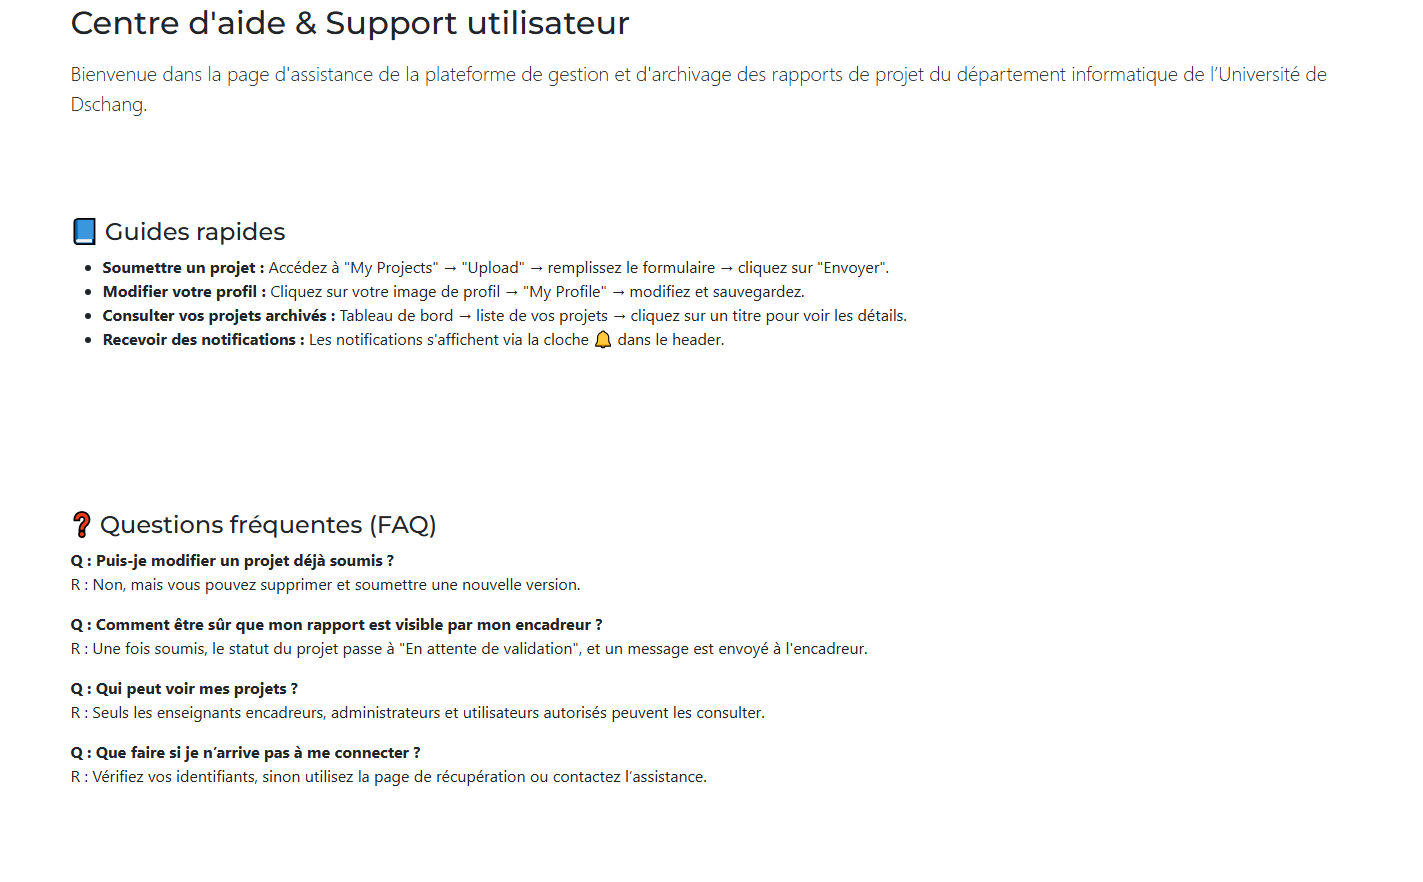
\includegraphics[width=0.7\textwidth]{images/page-aide.png}
        \caption{vue sur la page d'aide}
        \label{page d'aide}
    \end{figure}     
\medskip
\newline
Notre plateforme dispose également d'une page "Contact" accessible depuis l'entrée. Elle permet à un visiteur (personne n'ayant pas de compte) de s'enquérir autant qu'elle le souhaite à partir de ses informations. Voici un visuel de cette page:
        
        \begin{figure}[h!]
            \centering
            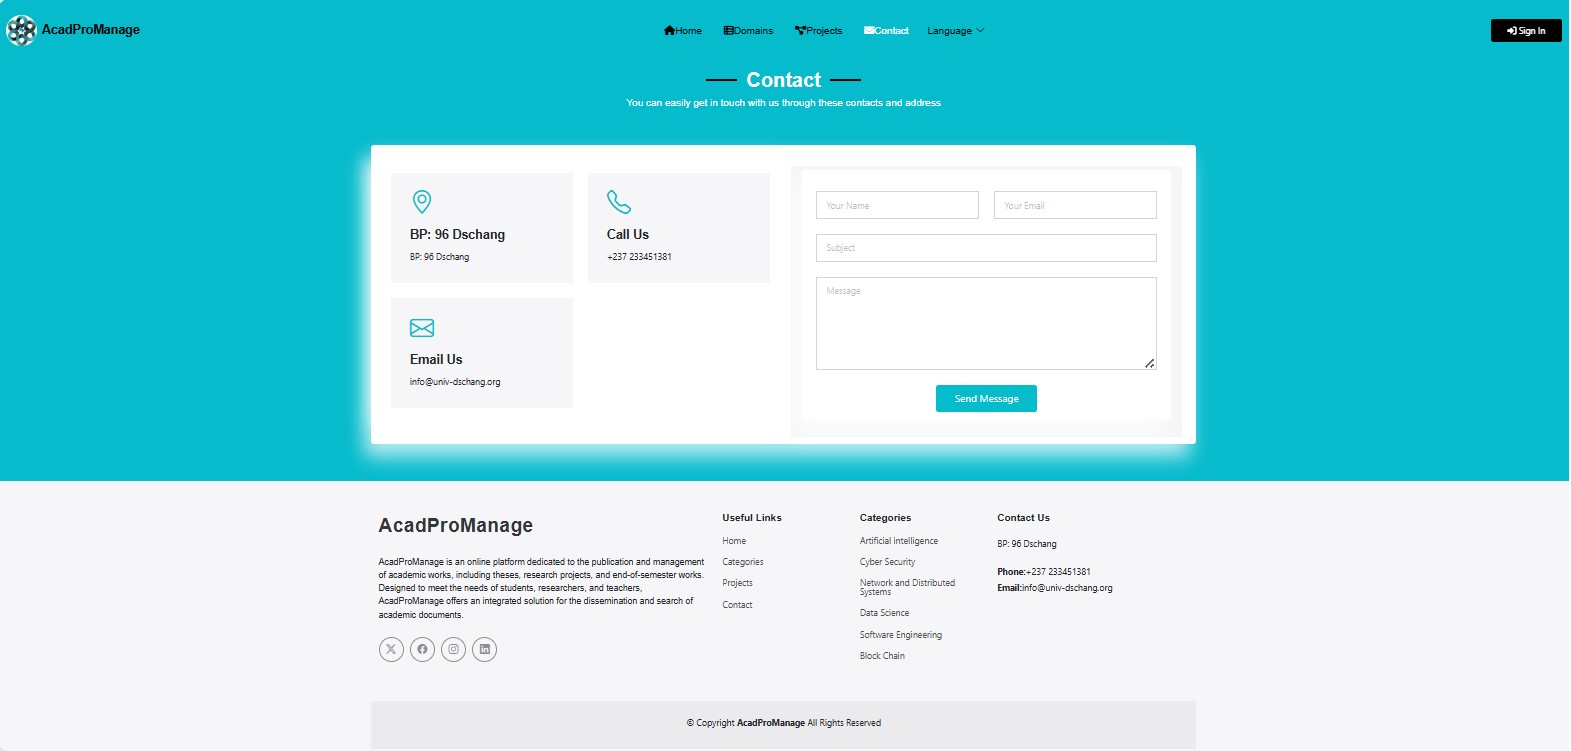
\includegraphics[width=0.7\textwidth]{images/page-contact.jpg}
            \caption{vue sur la page contact}
            \label{page contact}
        \end{figure}     
\newpage
{\fontsize{14}{16}\section*{Conclusion}}
\addcontentsline{toc}{section}{Conclusion}

Tout au long de ce travail, nous étions appelés à mettre sur pied un manuel d'orientation des utilisateurs dans la plateforme AcadProManage. Nous avons donc mis en exergue les fonctionnalités courantes dans l'application, ainsi que les fonctionnalités spécifiques à certains types d'utilisateurs. Il s'agit notamment du visiteur, de l'utilisateur ou étudiant et du superviseur ou enseignant. Parvenus au terme de notre travail, nous espérons grandement que ce manuel vous sera d'une aide véritable et constituera un tremplin pour votre épanouissement au sein de AcadPromanage. Toutefois, nous pouvons affirmer que ce petit guide conçu dans votre intérêt ne sera pas de la moindre utilité.
\end{document}
